% Options for packages loaded elsewhere
\PassOptionsToPackage{unicode}{hyperref}
\PassOptionsToPackage{hyphens}{url}
%
\documentclass[
  ignorenonframetext,
]{beamer}
\usepackage{pgfpages}
\setbeamertemplate{caption}[numbered]
\setbeamertemplate{caption label separator}{: }
\setbeamercolor{caption name}{fg=normal text.fg}
\beamertemplatenavigationsymbolsempty
% Prevent slide breaks in the middle of a paragraph
\widowpenalties 1 10000
\raggedbottom
\setbeamertemplate{part page}{
  \centering
  \begin{beamercolorbox}[sep=16pt,center]{part title}
    \usebeamerfont{part title}\insertpart\par
  \end{beamercolorbox}
}
\setbeamertemplate{section page}{
  \centering
  \begin{beamercolorbox}[sep=12pt,center]{part title}
    \usebeamerfont{section title}\insertsection\par
  \end{beamercolorbox}
}
\setbeamertemplate{subsection page}{
  \centering
  \begin{beamercolorbox}[sep=8pt,center]{part title}
    \usebeamerfont{subsection title}\insertsubsection\par
  \end{beamercolorbox}
}
\AtBeginPart{
  \frame{\partpage}
}
\AtBeginSection{
  \ifbibliography
  \else
    \frame{\sectionpage}
  \fi
}
\AtBeginSubsection{
  \frame{\subsectionpage}
}
\usepackage{lmodern}
\usepackage{amssymb,amsmath}
\usepackage{ifxetex,ifluatex}
\ifnum 0\ifxetex 1\fi\ifluatex 1\fi=0 % if pdftex
  \usepackage[T1]{fontenc}
  \usepackage[utf8]{inputenc}
  \usepackage{textcomp} % provide euro and other symbols
\else % if luatex or xetex
  \usepackage{unicode-math}
  \defaultfontfeatures{Scale=MatchLowercase}
  \defaultfontfeatures[\rmfamily]{Ligatures=TeX,Scale=1}
\fi
\usetheme[]{metropolis}
% Use upquote if available, for straight quotes in verbatim environments
\IfFileExists{upquote.sty}{\usepackage{upquote}}{}
\IfFileExists{microtype.sty}{% use microtype if available
  \usepackage[]{microtype}
  \UseMicrotypeSet[protrusion]{basicmath} % disable protrusion for tt fonts
}{}
\makeatletter
\@ifundefined{KOMAClassName}{% if non-KOMA class
  \IfFileExists{parskip.sty}{%
    \usepackage{parskip}
  }{% else
    \setlength{\parindent}{0pt}
    \setlength{\parskip}{6pt plus 2pt minus 1pt}}
}{% if KOMA class
  \KOMAoptions{parskip=half}}
\makeatother
\usepackage{xcolor}
\IfFileExists{xurl.sty}{\usepackage{xurl}}{} % add URL line breaks if available
\IfFileExists{bookmark.sty}{\usepackage{bookmark}}{\usepackage{hyperref}}
\hypersetup{
  pdftitle={Análise de imagem no Rstudio},
  pdfauthor={Ana Tércia, João, Laura Reis, Leonardo e Paulo},
  hidelinks,
  pdfcreator={LaTeX via pandoc}}
\urlstyle{same} % disable monospaced font for URLs
\newif\ifbibliography
\usepackage{color}
\usepackage{fancyvrb}
\newcommand{\VerbBar}{|}
\newcommand{\VERB}{\Verb[commandchars=\\\{\}]}
\DefineVerbatimEnvironment{Highlighting}{Verbatim}{commandchars=\\\{\}}
% Add ',fontsize=\small' for more characters per line
\usepackage{framed}
\definecolor{shadecolor}{RGB}{248,248,248}
\newenvironment{Shaded}{\begin{snugshade}}{\end{snugshade}}
\newcommand{\AlertTok}[1]{\textcolor[rgb]{0.94,0.16,0.16}{#1}}
\newcommand{\AnnotationTok}[1]{\textcolor[rgb]{0.56,0.35,0.01}{\textbf{\textit{#1}}}}
\newcommand{\AttributeTok}[1]{\textcolor[rgb]{0.77,0.63,0.00}{#1}}
\newcommand{\BaseNTok}[1]{\textcolor[rgb]{0.00,0.00,0.81}{#1}}
\newcommand{\BuiltInTok}[1]{#1}
\newcommand{\CharTok}[1]{\textcolor[rgb]{0.31,0.60,0.02}{#1}}
\newcommand{\CommentTok}[1]{\textcolor[rgb]{0.56,0.35,0.01}{\textit{#1}}}
\newcommand{\CommentVarTok}[1]{\textcolor[rgb]{0.56,0.35,0.01}{\textbf{\textit{#1}}}}
\newcommand{\ConstantTok}[1]{\textcolor[rgb]{0.00,0.00,0.00}{#1}}
\newcommand{\ControlFlowTok}[1]{\textcolor[rgb]{0.13,0.29,0.53}{\textbf{#1}}}
\newcommand{\DataTypeTok}[1]{\textcolor[rgb]{0.13,0.29,0.53}{#1}}
\newcommand{\DecValTok}[1]{\textcolor[rgb]{0.00,0.00,0.81}{#1}}
\newcommand{\DocumentationTok}[1]{\textcolor[rgb]{0.56,0.35,0.01}{\textbf{\textit{#1}}}}
\newcommand{\ErrorTok}[1]{\textcolor[rgb]{0.64,0.00,0.00}{\textbf{#1}}}
\newcommand{\ExtensionTok}[1]{#1}
\newcommand{\FloatTok}[1]{\textcolor[rgb]{0.00,0.00,0.81}{#1}}
\newcommand{\FunctionTok}[1]{\textcolor[rgb]{0.00,0.00,0.00}{#1}}
\newcommand{\ImportTok}[1]{#1}
\newcommand{\InformationTok}[1]{\textcolor[rgb]{0.56,0.35,0.01}{\textbf{\textit{#1}}}}
\newcommand{\KeywordTok}[1]{\textcolor[rgb]{0.13,0.29,0.53}{\textbf{#1}}}
\newcommand{\NormalTok}[1]{#1}
\newcommand{\OperatorTok}[1]{\textcolor[rgb]{0.81,0.36,0.00}{\textbf{#1}}}
\newcommand{\OtherTok}[1]{\textcolor[rgb]{0.56,0.35,0.01}{#1}}
\newcommand{\PreprocessorTok}[1]{\textcolor[rgb]{0.56,0.35,0.01}{\textit{#1}}}
\newcommand{\RegionMarkerTok}[1]{#1}
\newcommand{\SpecialCharTok}[1]{\textcolor[rgb]{0.00,0.00,0.00}{#1}}
\newcommand{\SpecialStringTok}[1]{\textcolor[rgb]{0.31,0.60,0.02}{#1}}
\newcommand{\StringTok}[1]{\textcolor[rgb]{0.31,0.60,0.02}{#1}}
\newcommand{\VariableTok}[1]{\textcolor[rgb]{0.00,0.00,0.00}{#1}}
\newcommand{\VerbatimStringTok}[1]{\textcolor[rgb]{0.31,0.60,0.02}{#1}}
\newcommand{\WarningTok}[1]{\textcolor[rgb]{0.56,0.35,0.01}{\textbf{\textit{#1}}}}
\usepackage{graphicx,grffile}
\makeatletter
\def\maxwidth{\ifdim\Gin@nat@width>\linewidth\linewidth\else\Gin@nat@width\fi}
\def\maxheight{\ifdim\Gin@nat@height>\textheight\textheight\else\Gin@nat@height\fi}
\makeatother
% Scale images if necessary, so that they will not overflow the page
% margins by default, and it is still possible to overwrite the defaults
% using explicit options in \includegraphics[width, height, ...]{}
\setkeys{Gin}{width=\maxwidth,height=\maxheight,keepaspectratio}
% Set default figure placement to htbp
\makeatletter
\def\fps@figure{htbp}
\makeatother
\setlength{\emergencystretch}{3em} % prevent overfull lines
\providecommand{\tightlist}{%
  \setlength{\itemsep}{0pt}\setlength{\parskip}{0pt}}
\setcounter{secnumdepth}{-\maxdimen} % remove section numbering
\metroset{numbering=none}
\usepackage{background}
\usepackage{TikZ}
\usepackage[absolute, overlay]{textpos}
\definecolor{shadecolor}{RGB}{240,240,240}

\renewcommand{\baselinestretch}{1.5}
\newcommand{\RefTb}[1]{\textbf{Tabela~\ref{#1}}}
\newcommand{\RefFg}[1]{\textbf{Figura~\ref{#1}}}
\newcommand{\blackbox}{\rule{1.5ex}{1.5ex}}
\newcommand{\lp}{\left(}
\newcommand{\rp}{\right)}
\newcommand{\lch}{\left\{}
\newcommand{\rch}{\right\}}
\newcommand{\lc}{\left[}
\newcommand{\rc}{\right]}
\newcommand{\I}{1\!\!1}
\newcommand{\fimteo}{\hfill\rule[.5mm]{1ex}{1ex}}
\newcommand{\bff}[1]{\boldsymbol{#1}}
\newcommand{\rhob}{\bff{\rho}}
\newcommand{\kappab}{\bff{\kappa}}
\newcommand{\alphab}{\bff{\alpha}}
\newcommand{\betab}{\bff{\beta}}
\newcommand{\thetab}{\bff{\theta}}
\newcommand{\mub}{\bff{\mu}}
\newcommand{\gammab}{\bff{\gamma}}
\newcommand{\Gammab}{\bff{\Gamma}}
\newcommand{\varphib}{\bff{\varphi}}
\newcommand{\etab}{\bff{\eta}}
\newcommand{\zetab}{\bff{\zeta}}
\newcommand{\psib}{\bff{\psi}}
\newcommand{\Psib}{\bff{\Psi}}
\newcommand{\omegab}{\bff{\omega}}
\newcommand{\Sigmab}{\bff{\Sigma}}
\newcommand{\taub}{\bff{\tau}}
\newcommand{\pib}{\bff{\pi}}
\newcommand{\lambdab}{\bff{\lambda}}
\newcommand{\Lambdab}{\bff{\Lambda}}
\newcommand{\Deltab}{\bff{\Delta}}
\newcommand{\deltab}{\bff{\delta}}
\newcommand{\Imat}{\bff{\mathcal{I}}}
\newcommand{\phib}{\bff{\phi}}
\newcommand{\umb}{\bff{1}}
\newcommand{\zb}{\bff{0}}
\newcommand{\Ub}{\bff{U}}
\newcommand{\Cb}{\bff{C}}
\newcommand{\Sbl}{\bff{S}}
\newcommand{\sbl}{\bff{s}}
\newcommand{\Abl}{\bff{A}}
\newcommand{\Tb}{\bff{T}}
\newcommand{\Yb}{\bff{Y}}
\newcommand{\yb}{\bff{y}}
\newcommand{\Nb}{\bff{N}}
\newcommand{\nb}{\bff{n}}
\newcommand{\Ib}{\bff{I}}
\newcommand{\Hb}{\bff{H}}
\newcommand{\hb}{\bff{h}}
\newcommand{\Jb}{\bff{J}}
\newcommand{\Kb}{\bff{K}}
\newcommand{\Hbl}{\bff{H}}
\newcommand{\lb}{\bff{l}}
\newcommand{\Lb}{\bff{L}}
\newcommand{\xb}{\bff{x}}
\newcommand{\Xb}{\bff{X}}
\newcommand{\Wb}{\bff{W}}
\newcommand{\mb}{\bff{m}}
\newcommand{\Mb}{\bff{M}}
\newcommand{\Ab}{\bff{A}}
\newcommand{\ab}{\bff{a}}
\newcommand{\Bb}{\bff{B}}
\newcommand{\Pb}{\bff{P}}
\newcommand{\db}{\bff{d}}
\newcommand{\vb}{\bff{v}}
\newcommand{\tb}{\bff{t}}
\newcommand{\Vb}{\bff{V}}
\newcommand{\Db}{\bff{D}}
\newcommand{\Eb}{\bff{E}}
\newcommand{\Fb}{\bff{F}}
\newcommand{\fb}{\bff{f}}
\newcommand{\Rb}{\bff{R}}
\newcommand{\Zbl}{\bff{Z}}
\newcommand{\zbl}{\bff{z}}
\newcommand{\rb}{\bff{r}}
\newcommand{\bdot}{\bff{.}}
\newcommand{\varthetab}{\bff{\vartheta}}
\newcommand{\ini}{\noindent}
\newcommand{\inic}{\hspace{5.5mm}}
\newcommand{\mU}{\mathcal{U}}
\newcommand{\mS}{\mathcal{S}}
\newcommand{\EM}{\mathcal{E}}
\newcommand{\VM}{\mathcal{V}}
\newcommand{\Real}{\mathcal{R}}
\newcommand{\SA}{\mathcal{A}}
\newcommand{\MP}{\mathcal{P}}
\newcommand{\mpp}{{\it {p}}}
\newcommand{\ds}{\displaystyle}
\newcommand{\wthetab}{\widehat{\thetab}}
\newcommand{\wpib}{\widehat{\pib}}


\newcommand{\beq}{\begin{eqnarray}}
\newcommand{\eeq}{\end{eqnarray}}
\newcommand{\beqq}{\begin{eqnarray*}}
\newcommand{\eeqq}{\end{eqnarray*}}
\newcommand\mycom[2]{\genfrac{}{}{0pt}{}{#1}{#2}}

\title{Análise de imagem no Rstudio}
\author{Ana Tércia, João, Laura Reis, Leonardo e Paulo}
\date{20 de novembro de 2019}

\begin{document}
\frame{\titlepage}

\begin{frame}{Tipos de imagens (Bitmap)}
\protect\hypertarget{tipos-de-imagens-bitmap}{}

\small

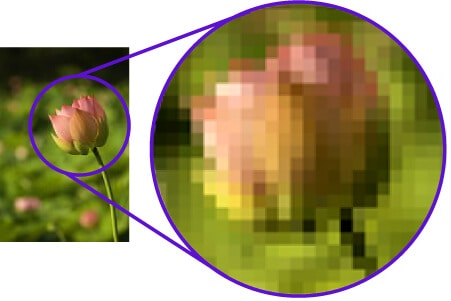
\includegraphics[width=4.4in]{IMAGENS/BITMAP}

\begin{center}
\tiny{}
\end{center}

\end{frame}

\begin{frame}{Tipos de imagens (Vetorial)}
\protect\hypertarget{tipos-de-imagens-vetorial}{}

\small

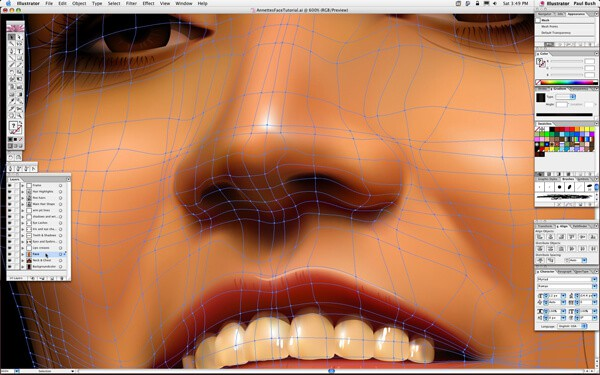
\includegraphics[width=4.4in]{IMAGENS/VETORIAL}

\begin{center}
\tiny{}
\end{center}

\end{frame}

\begin{frame}{Formatos de imagens}
\protect\hypertarget{formatos-de-imagens}{}

\small

\begin{itemize}
    \item TIFF
    \item BMP
    \item JPEG
    \item PNG
    \item SVG
    \item GIF
    \item PDF
    \item EPS
\end{itemize}

\end{frame}

\begin{frame}{A importância de análise de imagens}
\protect\hypertarget{a-importuxe2ncia-de-anuxe1lise-de-imagens}{}

\small

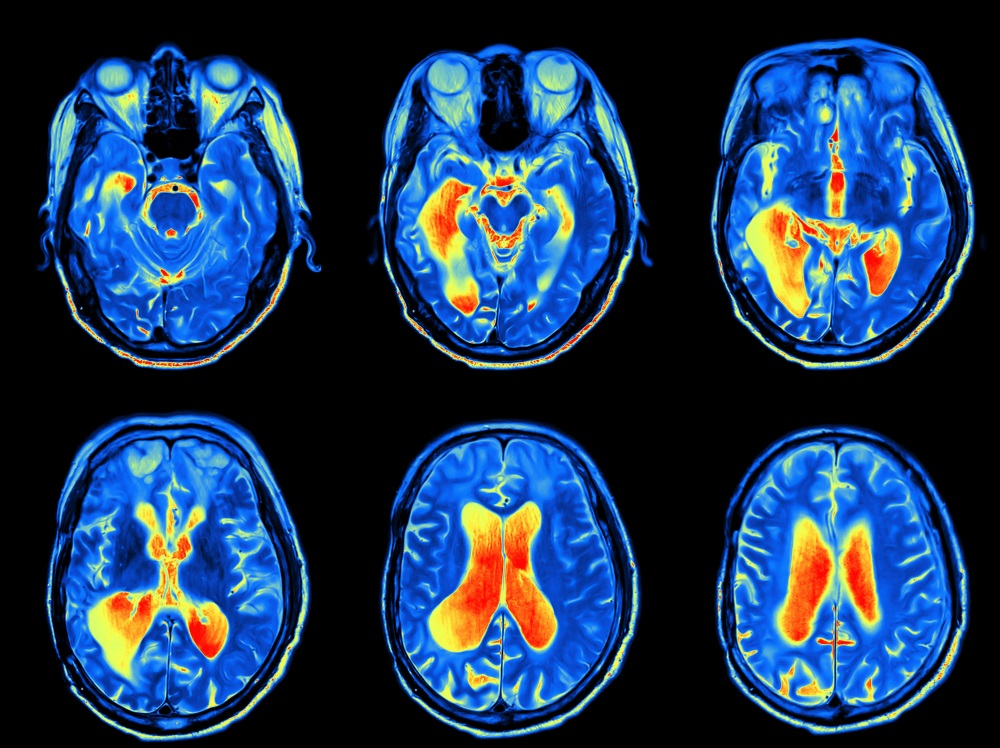
\includegraphics[width=4.4in]{IMAGENS/raiox}

\begin{center}
\tiny{}
\end{center}

\end{frame}

\begin{frame}{A importância de análise de imagens}
\protect\hypertarget{a-importuxe2ncia-de-anuxe1lise-de-imagens-1}{}

\small

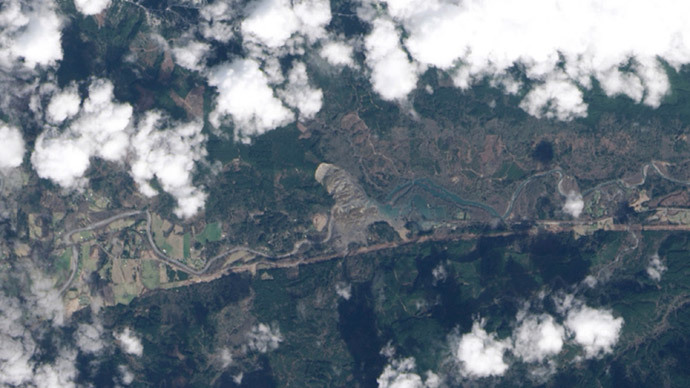
\includegraphics[width=4.4in]{IMAGENS/satelite}

\begin{center}
\tiny{}
\end{center}

\end{frame}

\begin{frame}{A importância de análise de imagens}
\protect\hypertarget{a-importuxe2ncia-de-anuxe1lise-de-imagens-2}{}

\small

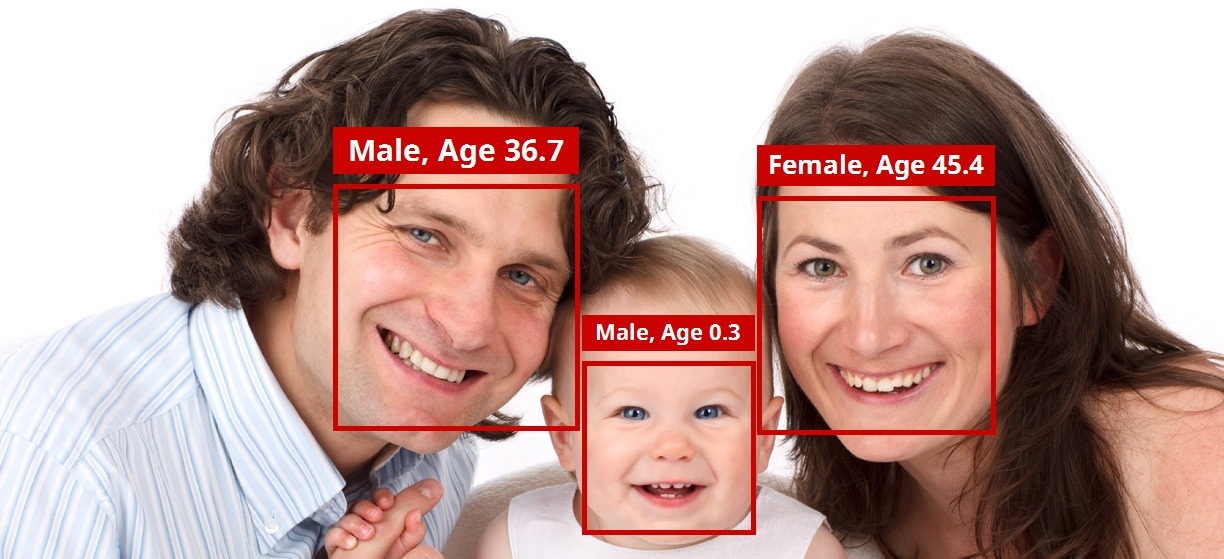
\includegraphics[width=4.4in]{IMAGENS/facial}

\begin{center}
\tiny{}
\end{center}

\end{frame}

\begin{frame}{Como os pacotes lêem as imagens?}
\protect\hypertarget{como-os-pacotes-luxeaem-as-imagens}{}

\small

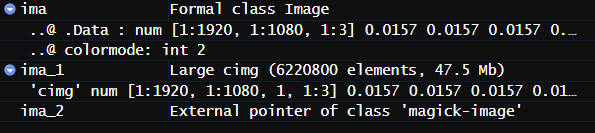
\includegraphics[width=4.6in]{IMAGENS/R_le}

\begin{center}
\tiny{}
\end{center}

\end{frame}

\begin{frame}[fragile]{Pacotes}
\protect\hypertarget{pacotes}{}

\small

Oos principais pacotes para manipulação de imagem são:

\begin{Shaded}
\begin{Highlighting}[]
\KeywordTok{require}\NormalTok{(}\StringTok{"BiocManager"}\NormalTok{) }
\KeywordTok{require}\NormalTok{(}\StringTok{"EBImage"}\NormalTok{) }

\KeywordTok{require}\NormalTok{(}\StringTok{"imager"}\NormalTok{) }

\KeywordTok{require}\NormalTok{(}\StringTok{"magick"}\NormalTok{) }
\end{Highlighting}
\end{Shaded}

\end{frame}

\begin{frame}{Importação e vizualização de imagens:}
\protect\hypertarget{importauxe7uxe3o-e-vizualizauxe7uxe3o-de-imagens}{}

\small

\begin{itemize}
\tightlist
\item
  EBImage:
\end{itemize}

.ima \textless- readImage(``C:/Users/nick\_/Downloads/897207.jpg'')
.display(ima)

\begin{itemize}
\tightlist
\item
  Imager:
\end{itemize}

.ima\_1 \textless- load.image(``C:/Users/nick\_/Downloads/897207.jpg'')
.plot(ima\_1)

\begin{itemize}
\tightlist
\item
  Magick:
\end{itemize}

.ima\_2 \textless- image\_read(``C:/Users/nick\_/Downloads/897207.jpg'')
.print(ima\_2)

\end{frame}

\begin{frame}[fragile]{Mudar dimensões}
\protect\hypertarget{mudar-dimensuxf5es}{}

\small

\begin{Shaded}
\begin{Highlighting}[]
\KeywordTok{library}\NormalTok{(rsvg)}
\NormalTok{queremos <-}\StringTok{ }\KeywordTok{image_read_svg}\NormalTok{(}
  \StringTok{'https://s3.amazonaws.com/wd-static/static_v1/pt/logo.svg'}\NormalTok{)}
\NormalTok{queremos}
\end{Highlighting}
\end{Shaded}


\includegraphics[width=3.89in]{SLIDES_files/figure-beamer/2-1}

\end{frame}

\begin{frame}[fragile]{Mudar dimensões}
\protect\hypertarget{mudar-dimensuxf5es-1}{}

\small

\begin{Shaded}
\begin{Highlighting}[]
\NormalTok{queremos2 <-}\StringTok{ }\KeywordTok{image_read_svg}\NormalTok{(}
  \StringTok{'https://s3.amazonaws.com/wd-static/static_v1/pt/logo.svg'}\NormalTok{,}
  \DataTypeTok{width =} \DecValTok{210}\NormalTok{) }\CommentTok{# 220 = width,}
               \CommentTok{# 220x = height}
\NormalTok{queremos2}
\end{Highlighting}
\end{Shaded}


\includegraphics[width=2.92in]{SLIDES_files/figure-beamer/2.1-1}

\end{frame}

\begin{frame}[fragile]{Mudar dimensões}
\protect\hypertarget{mudar-dimensuxf5es-2}{}

\small

\begin{Shaded}
\begin{Highlighting}[]
\NormalTok{queremos_redimensionado1 <-}\StringTok{ }\KeywordTok{image_scale}\NormalTok{(queremos, }\StringTok{"210x42"}\NormalTok{)}
\KeywordTok{image_info}\NormalTok{(queremos_redimensionado1)}
\end{Highlighting}
\end{Shaded}

\begin{verbatim}
##   format width height colorspace matte filesize density
## 1    PNG   210     41       sRGB  TRUE        0   72x72
\end{verbatim}

\begin{Shaded}
\begin{Highlighting}[]
\NormalTok{queremos_redimensionado2 <-}\StringTok{ }\KeywordTok{image_scale}\NormalTok{(queremos, }\StringTok{"210x40"}\NormalTok{)}
\KeywordTok{image_info}\NormalTok{(queremos_redimensionado2)}
\end{Highlighting}
\end{Shaded}

\begin{verbatim}
##   format width height colorspace matte filesize density
## 1    PNG   207     40       sRGB  TRUE        0   72x72
\end{verbatim}

\end{frame}

\begin{frame}[fragile]{Converter ou salvar em formatos desejados}
\protect\hypertarget{converter-ou-salvar-em-formatos-desejados}{}

\small

\begin{Shaded}
\begin{Highlighting}[]
\NormalTok{tigre_convertido <-}\StringTok{ }\KeywordTok{image_convert}\NormalTok{(queremos, }\StringTok{"jpeg"}\NormalTok{)}
\KeywordTok{image_info}\NormalTok{(tigre_convertido) }\CommentTok{# Retorna o formato da imagem}
\end{Highlighting}
\end{Shaded}

\begin{verbatim}
##   format width height colorspace matte filesize density
## 1   JPEG   280     54       sRGB  TRUE        0   72x72
\end{verbatim}

\begin{Shaded}
\begin{Highlighting}[]
\KeywordTok{image_write}\NormalTok{(queremos, }\DataTypeTok{path =} \StringTok{"queremos.png"}\NormalTok{, }\DataTypeTok{format =} \StringTok{"png"}\NormalTok{)}
\end{Highlighting}
\end{Shaded}

\end{frame}

\begin{frame}[fragile]{Imagens para manipulação}
\protect\hypertarget{imagens-para-manipulauxe7uxe3o}{}

\small

\begin{Shaded}
\begin{Highlighting}[]
\NormalTok{patrik <-}\StringTok{ }\KeywordTok{image_read}\NormalTok{(}\StringTok{"IMAGENS/patrik.png"}\NormalTok{)}
\end{Highlighting}
\end{Shaded}


\includegraphics[width=3.2in]{IMAGENS/patrik}

\begin{center}
\tiny{}
\end{center}

\end{frame}

\begin{frame}[fragile]{Imagens para manipulação}
\protect\hypertarget{imagens-para-manipulauxe7uxe3o-1}{}

\small

\begin{Shaded}
\begin{Highlighting}[]
\NormalTok{bigdata <-}\StringTok{ }\KeywordTok{image_read}\NormalTok{(}\StringTok{'IMAGENS/bigdata.jpg'}\NormalTok{)}
\end{Highlighting}
\end{Shaded}


\includegraphics[width=3.7in]{IMAGENS/bigdata}

\begin{center}
\tiny{}
\end{center}

\end{frame}

\begin{frame}[fragile]{Imagens para manipulação}
\protect\hypertarget{imagens-para-manipulauxe7uxe3o-2}{}

\small

\begin{Shaded}
\begin{Highlighting}[]
\NormalTok{logo <-}\StringTok{ }\KeywordTok{image_read}\NormalTok{(}\StringTok{'IMAGENS/Rlogo.png'}\NormalTok{)}
\end{Highlighting}
\end{Shaded}


\includegraphics[width=3.4in]{IMAGENS/Rlogo}

\begin{center}
\tiny{}
\end{center}

\end{frame}

\begin{frame}{Girar e modificar}
\protect\hypertarget{girar-e-modificar}{}

\small

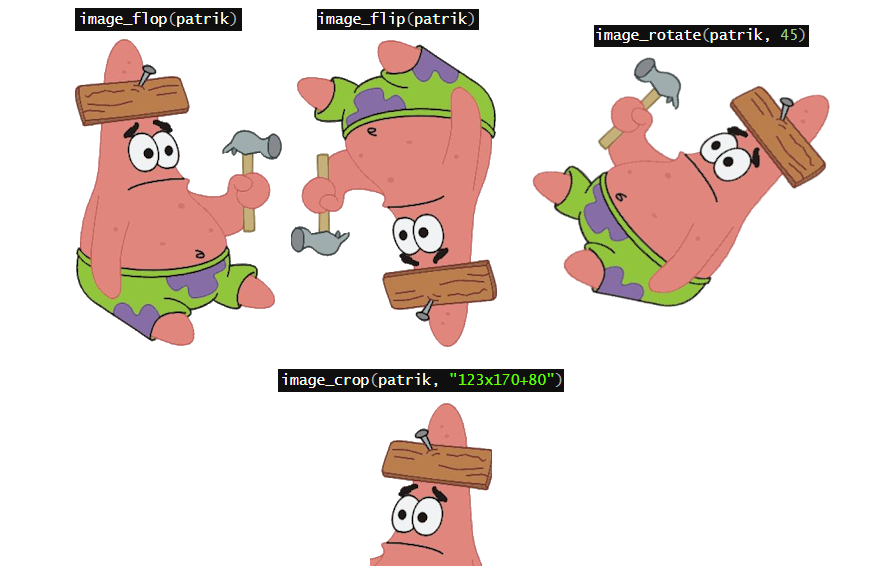
\includegraphics[width=4.6in]{IMAGENS/girar_modificar}

\begin{center}
\tiny{}
\end{center}

\end{frame}

\begin{frame}{Alguns tipos de filtros}
\protect\hypertarget{alguns-tipos-de-filtros}{}

\small

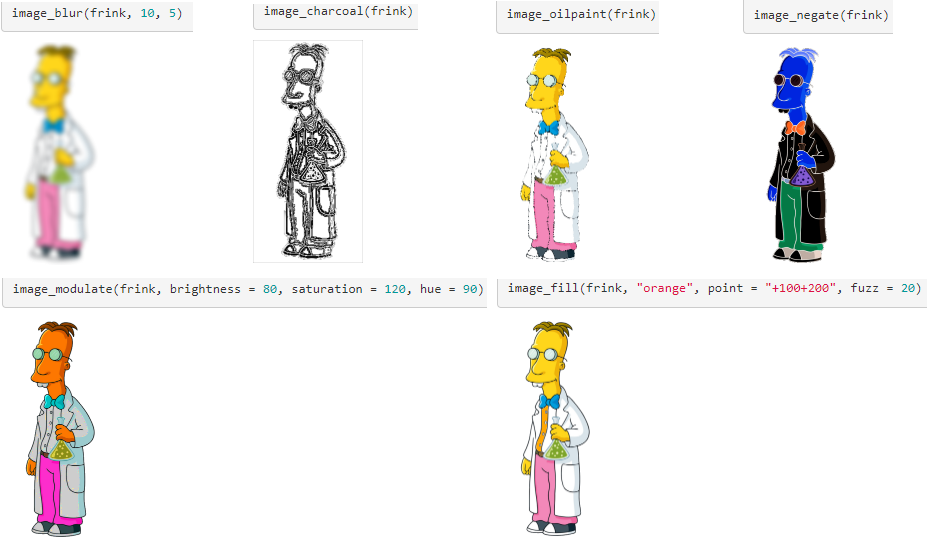
\includegraphics[width=4.4in]{IMAGENS/filtros}

\begin{center}
\tiny{}
\end{center}

\end{frame}

\begin{frame}[fragile]{Imagens sobrepostas}
\protect\hypertarget{imagens-sobrepostas}{}

\small

\begin{Shaded}
\begin{Highlighting}[]
\NormalTok{img <-}\StringTok{ }\KeywordTok{c}\NormalTok{(bigdata, logo, patrik)}
\NormalTok{img <-}\StringTok{ }\KeywordTok{image_scale}\NormalTok{(img, }\StringTok{"300x300"}\NormalTok{)}
\KeywordTok{image_info}\NormalTok{(img)}
\end{Highlighting}
\end{Shaded}

\begin{verbatim}
##   format width height colorspace matte filesize density
## 1   JPEG   300    207       sRGB FALSE        0   96x96
## 2    PNG   300    232       sRGB  TRUE        0   72x72
## 3    PNG   203    300       sRGB  TRUE        0   72x72
\end{verbatim}

\end{frame}

\begin{frame}{Imagens sobrepostas}
\protect\hypertarget{imagens-sobrepostas-1}{}

\small

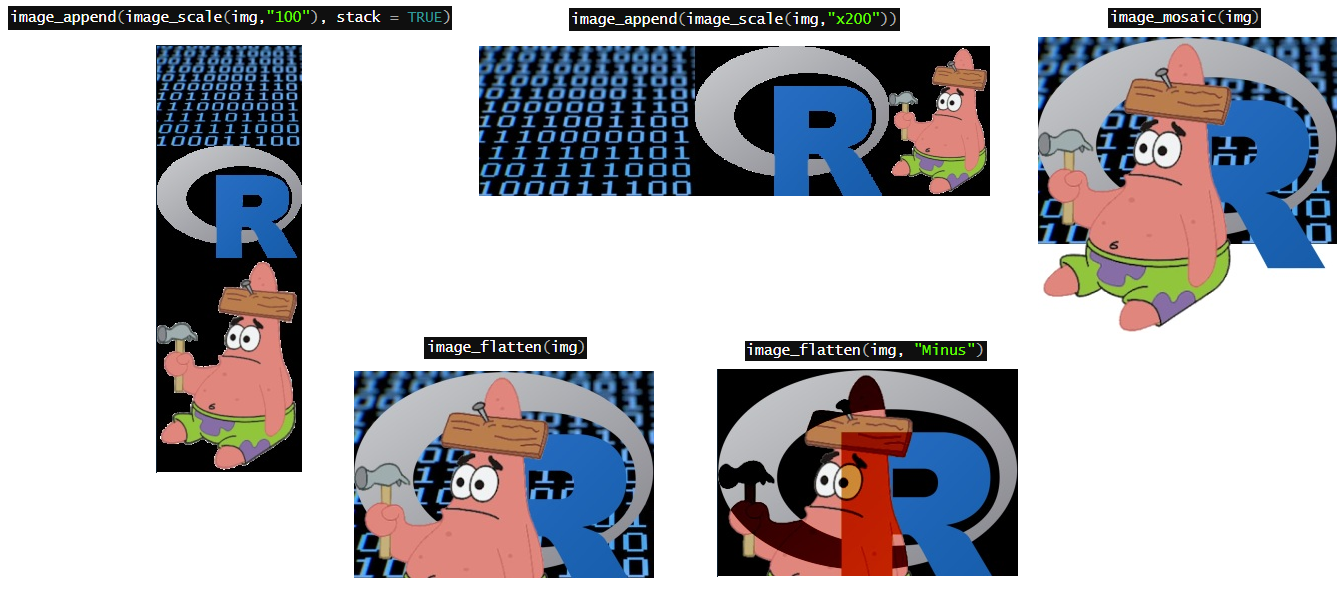
\includegraphics[width=4.6in]{IMAGENS/juntar_sobrepor}

\begin{center}
\tiny{}
\end{center}

\end{frame}

\begin{frame}[fragile]{Imagens sobrepostas}
\protect\hypertarget{imagens-sobrepostas-2}{}

\begin{Shaded}
\begin{Highlighting}[]
\NormalTok{bigdatapatrik <-}\StringTok{ }\KeywordTok{image_scale}\NormalTok{(}\KeywordTok{image_rotate}\NormalTok{(}
  \KeywordTok{image_background}\NormalTok{(patrik, }\StringTok{"none"}\NormalTok{), }\DecValTok{300}\NormalTok{), }\StringTok{"x260"}\NormalTok{)}
\NormalTok{juntos <-}\KeywordTok{image_composite}\NormalTok{(}\KeywordTok{image_scale}\NormalTok{(}
\NormalTok{  bigdata, }\StringTok{"x330"}\NormalTok{), bigdatapatrik, }\DataTypeTok{offset =} \StringTok{"+150+70"}\NormalTok{)}
\KeywordTok{image_write}\NormalTok{(juntos, }\DataTypeTok{path =} \StringTok{"juntos.png"}\NormalTok{, }\DataTypeTok{format =} \StringTok{"png"}\NormalTok{)}
\end{Highlighting}
\end{Shaded}

\end{frame}

\begin{frame}{Imagens sobrepostas}
\protect\hypertarget{imagens-sobrepostas-3}{}

\small


\includegraphics[width=4.4in]{juntos}

\begin{center}
\tiny{}
\end{center}

\end{frame}

\begin{frame}{Utilidade em gráficos}
\protect\hypertarget{utilidade-em-gruxe1ficos}{}

\small

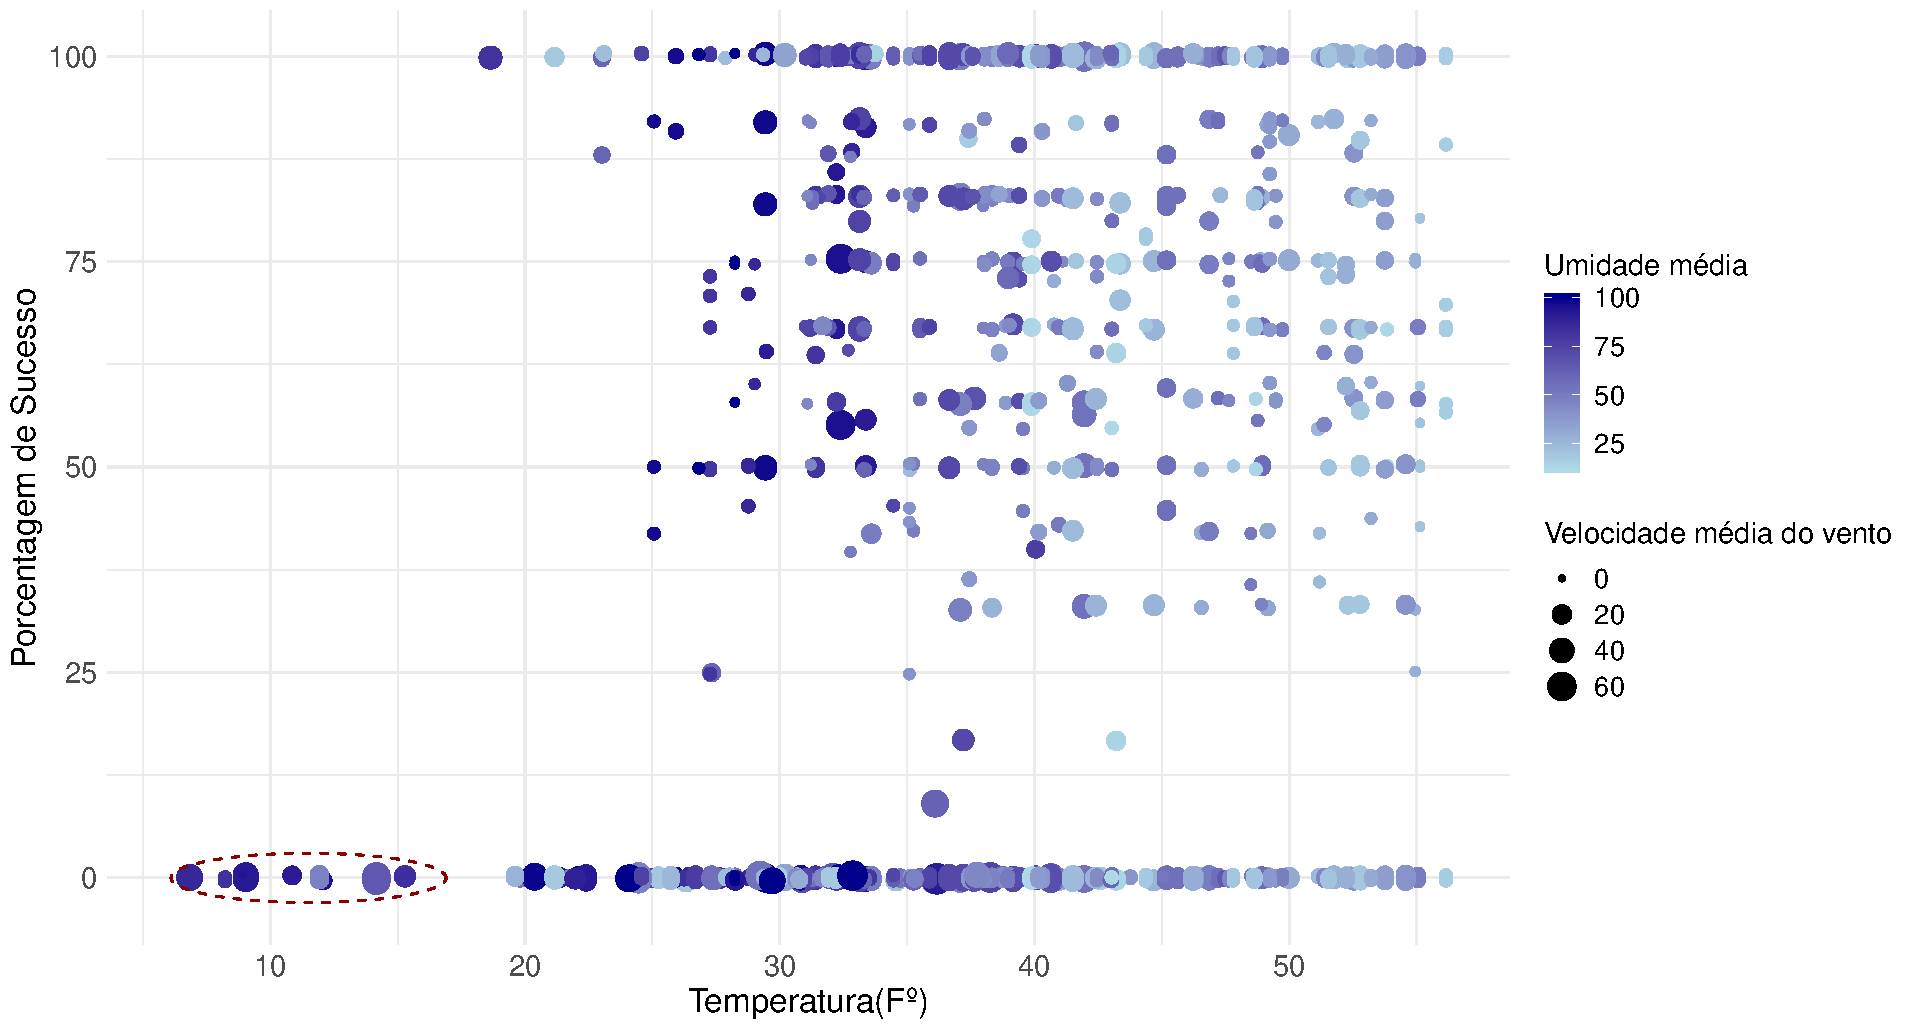
\includegraphics[width=4.4in]{PSxTEMP}

\begin{center}
\tiny{}
\end{center}

\end{frame}

\begin{frame}[fragile]{Utilidade para sobreposição de imagens}
\protect\hypertarget{utilidade-para-sobreposiuxe7uxe3o-de-imagens}{}

\begin{Shaded}
\begin{Highlighting}[]
\NormalTok{graph <-}\StringTok{ }\KeywordTok{image_read}\NormalTok{(}\StringTok{"IMAGENS/Rplot1.png"}\NormalTok{)}
\NormalTok{temp <-}\StringTok{ }\KeywordTok{image_read}\NormalTok{(}\StringTok{"IMAGENS/low_temp.png"}\NormalTok{)}
\NormalTok{temp_graph <-}\StringTok{ }\KeywordTok{image_scale}\NormalTok{(}\KeywordTok{image_rotate}\NormalTok{(}\KeywordTok{image_background}\NormalTok{(}
\NormalTok{  temp, }\StringTok{"none"}\NormalTok{), }\DecValTok{340}\NormalTok{), }\StringTok{"x50"}\NormalTok{)}
\NormalTok{temp_graph}
\end{Highlighting}
\end{Shaded}


\includegraphics[width=0.69in]{SLIDES_files/figure-beamer/6-1}

\begin{Shaded}
\begin{Highlighting}[]
\NormalTok{juntos_}\DecValTok{2}\NormalTok{ <-}\KeywordTok{image_composite}\NormalTok{(}\KeywordTok{image_scale}\NormalTok{(}
\NormalTok{  graph, }\StringTok{"x600"}\NormalTok{), temp_graph, }\DataTypeTok{offset =} \StringTok{"+150+440"}\NormalTok{)}
\KeywordTok{image_write}\NormalTok{(juntos_}\DecValTok{2}\NormalTok{, }\DataTypeTok{path =} \StringTok{"juntos2.pdf"}\NormalTok{,}
            \DataTypeTok{format =} \StringTok{"pdf"}\NormalTok{)}
\end{Highlighting}
\end{Shaded}

\end{frame}

\begin{frame}{Utilidade para sobreposição de imagens}
\protect\hypertarget{utilidade-para-sobreposiuxe7uxe3o-de-imagens-1}{}

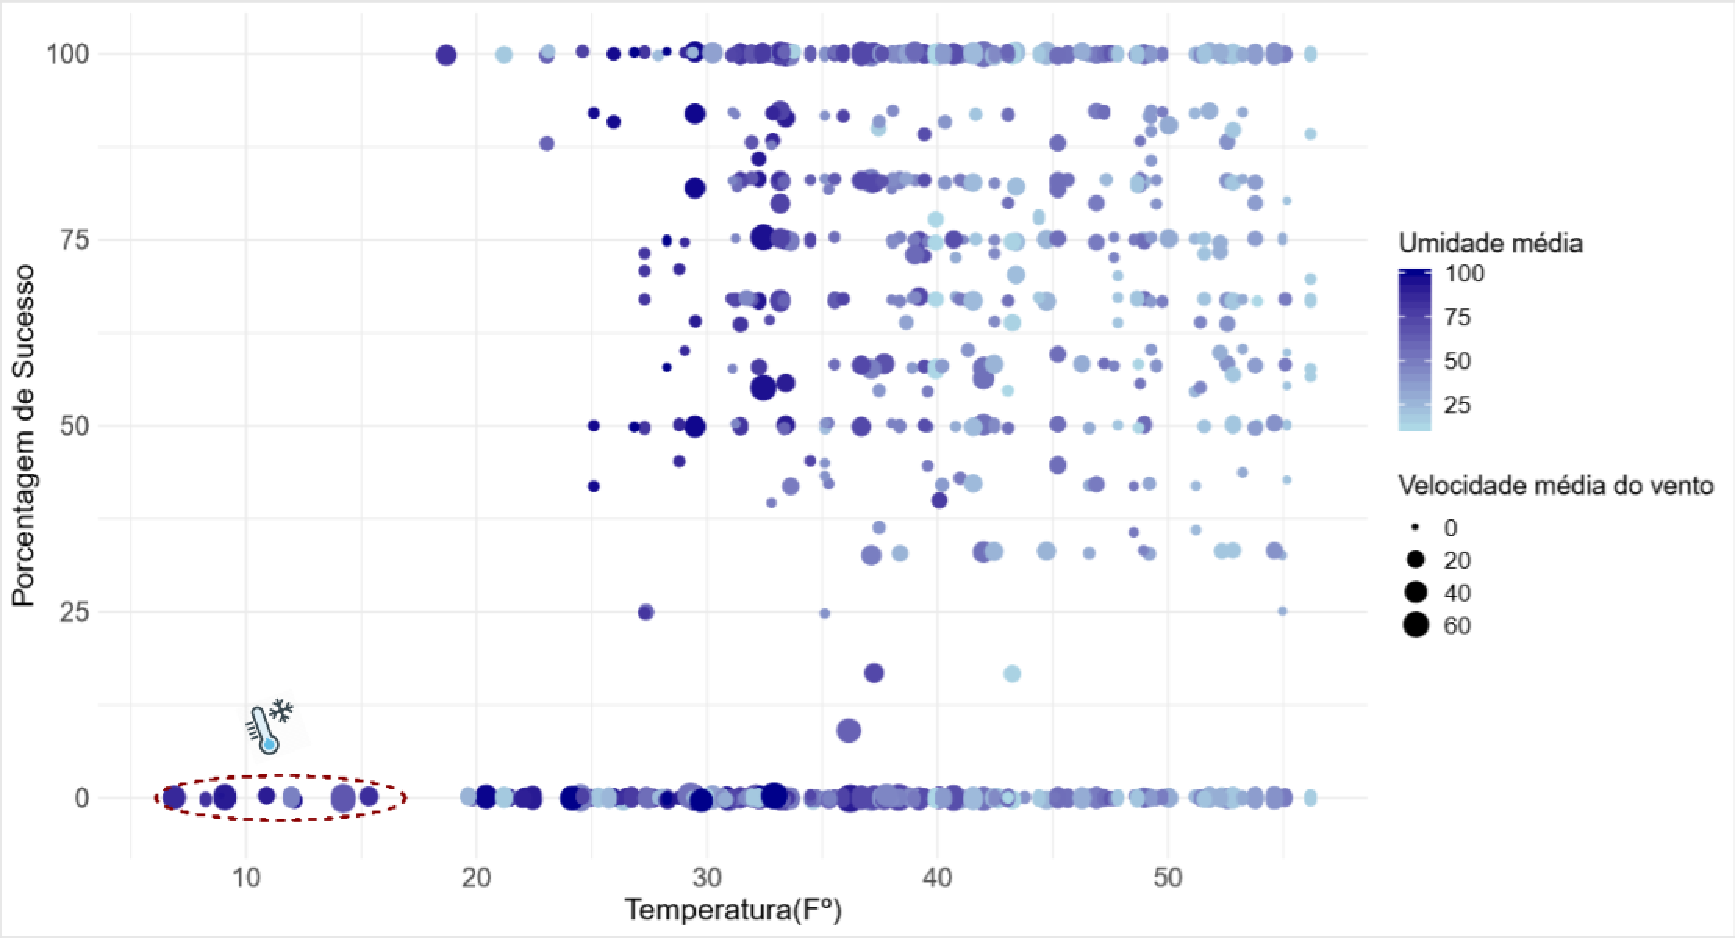
\includegraphics[width=4.4in]{juntos2}

\begin{center}
\tiny{}
\end{center}

\end{frame}

\begin{frame}[fragile]{Anotações em imagens}
\protect\hypertarget{anotauxe7uxf5es-em-imagens}{}

\begin{Shaded}
\begin{Highlighting}[]
\NormalTok{patrik_anot <-}\StringTok{ }\KeywordTok{image_annotate}\NormalTok{(patrik, }\StringTok{"Aqui"}\NormalTok{, }\DataTypeTok{size =} \DecValTok{21}\NormalTok{,}
                             \DataTypeTok{color =} \StringTok{"red"}\NormalTok{,}
                             \DataTypeTok{boxcolor =} \StringTok{"black"}\NormalTok{,}
                             \DataTypeTok{degrees =} \DecValTok{10}\NormalTok{, }
                             \DataTypeTok{location =} \StringTok{"+120+50"}\NormalTok{)}

\NormalTok{patrik_anot <-}\StringTok{ }\KeywordTok{image_scale}\NormalTok{(patrik_anot, }\StringTok{"x350"}\NormalTok{)}

\KeywordTok{image_write}\NormalTok{(patrik_anot, }\DataTypeTok{path =} \StringTok{"patrik_anot.png"}\NormalTok{,}
            \DataTypeTok{format =} \StringTok{"png"}\NormalTok{)}
\end{Highlighting}
\end{Shaded}

\end{frame}

\begin{frame}{Anotações em imagens}
\protect\hypertarget{anotauxe7uxf5es-em-imagens-1}{}


\includegraphics[width=3.6in]{patrik_anot}

\begin{center}
\tiny{}
\end{center}

\end{frame}

\begin{frame}{Como retirar pontos de um gráfico sem seu código?}
\protect\hypertarget{como-retirar-pontos-de-um-gruxe1fico-sem-seu-cuxf3digo}{}

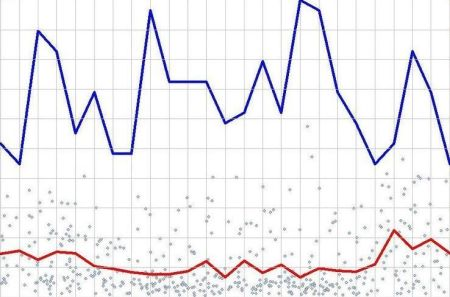
\includegraphics[width=4.4in]{IMAGENS/grafico_ponto}

\begin{center}
\tiny{}
\end{center}

\end{frame}

\begin{frame}[fragile]{Como retirar pontos de um gráfico sem seu
código?}
\protect\hypertarget{como-retirar-pontos-de-um-gruxe1fico-sem-seu-cuxf3digo-1}{}

\begin{Shaded}
\begin{Highlighting}[]
\KeywordTok{library}\NormalTok{(tidyverse)}
\NormalTok{im <-}\StringTok{ }\KeywordTok{image_read}\NormalTok{(}\StringTok{"IMAGENS/grafico_ponto.jpg"}\NormalTok{)}
\NormalTok{im_proc <-}\StringTok{ }\NormalTok{im }\OperatorTok
\StringTok{    }\KeywordTok{image_channel}\NormalTok{(}\StringTok{"saturation"}\NormalTok{)}
\KeywordTok{image_write}\NormalTok{(im_proc, }\DataTypeTok{path =} \StringTok{"IMAGENS/grafico_ponto1.png"}\NormalTok{,}
            \DataTypeTok{format =} \StringTok{"png"}\NormalTok{)}
\end{Highlighting}
\end{Shaded}

\end{frame}

\begin{frame}{Como retirar pontos de um gráfico sem seu código?}
\protect\hypertarget{como-retirar-pontos-de-um-gruxe1fico-sem-seu-cuxf3digo-2}{}

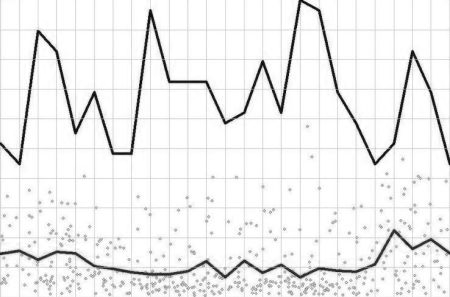
\includegraphics[width=4.4in]{IMAGENS/grafico_ponto1}

\begin{center}
\tiny{}
\end{center}

\end{frame}

\begin{frame}[fragile]{Como retirar pontos de um gráfico sem seu
código?}
\protect\hypertarget{como-retirar-pontos-de-um-gruxe1fico-sem-seu-cuxf3digo-3}{}

\small

\begin{Shaded}
\begin{Highlighting}[]
\NormalTok{im_proc2 <-}\StringTok{ }\NormalTok{im_proc }\OperatorTok
\StringTok{    }\KeywordTok{image_threshold}\NormalTok{(}\StringTok{"white"}\NormalTok{, }\StringTok{"30%"}\NormalTok{)}
\KeywordTok{image_write}\NormalTok{(im_proc2, }\DataTypeTok{path =} \StringTok{"IMAGENS/grafico_ponto2.png"}\NormalTok{,}
            \DataTypeTok{format =} \StringTok{"png"}\NormalTok{)}
\end{Highlighting}
\end{Shaded}

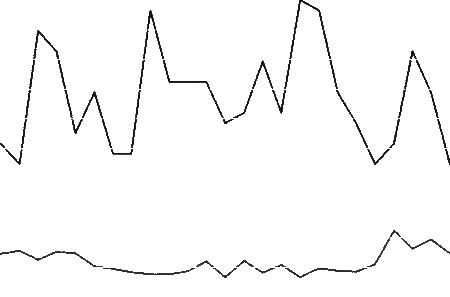
\includegraphics[width=3.6in]{IMAGENS/grafico_ponto2}

\begin{center}
\tiny{}
\end{center}

\end{frame}

\begin{frame}[fragile]{Como retirar pontos de um gráfico sem seu
código?}
\protect\hypertarget{como-retirar-pontos-de-um-gruxe1fico-sem-seu-cuxf3digo-4}{}

\small

\begin{Shaded}
\begin{Highlighting}[]
\NormalTok{im_proc3 <-}\StringTok{ }\NormalTok{im_proc2 }\OperatorTok
\StringTok{    }\KeywordTok{image_negate}\NormalTok{()}
\KeywordTok{image_write}\NormalTok{(im_proc3, }\DataTypeTok{path =} \StringTok{"IMAGENS/grafico_ponto3.png"}\NormalTok{,}
            \DataTypeTok{format =} \StringTok{"png"}\NormalTok{)}
\end{Highlighting}
\end{Shaded}

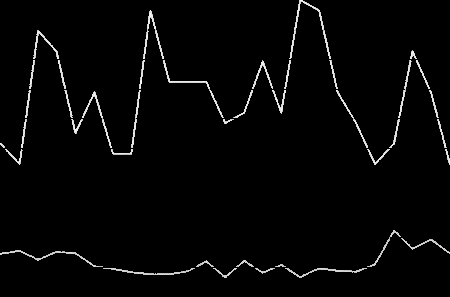
\includegraphics[width=3.6in]{IMAGENS/grafico_ponto3}

\begin{center}
\tiny{}
\end{center}

\end{frame}

\begin{frame}[fragile]{Como retirar pontos de um gráfico sem seu
código?}
\protect\hypertarget{como-retirar-pontos-de-um-gruxe1fico-sem-seu-cuxf3digo-5}{}

\small

\begin{Shaded}
\begin{Highlighting}[]
\KeywordTok{require}\NormalTok{(tidyverse)}
\NormalTok{dat <-}\StringTok{ }\KeywordTok{image_data}\NormalTok{(im_proc3)[}\DecValTok{1}\NormalTok{,,] }\OperatorTok
\StringTok{    }\KeywordTok{as.data.frame}\NormalTok{() }\OperatorTok
\StringTok{    }\KeywordTok{mutate}\NormalTok{(}\DataTypeTok{Row =} \DecValTok{1}\OperatorTok{:}\KeywordTok{nrow}\NormalTok{(.)) }\OperatorTok
\StringTok{    }\KeywordTok{select}\NormalTok{(Row, }\KeywordTok{everything}\NormalTok{()) }\OperatorTok
\StringTok{    }\KeywordTok{mutate_all}\NormalTok{(as.character) }\OperatorTok
\StringTok{    }\KeywordTok{gather}\NormalTok{(}\DataTypeTok{key =}\NormalTok{ Column, }\DataTypeTok{value =}\NormalTok{ value, }\DecValTok{2}\OperatorTok{:}\KeywordTok{ncol}\NormalTok{(.)) }\OperatorTok
\StringTok{    }\KeywordTok{mutate}\NormalTok{(}\DataTypeTok{Column =} \KeywordTok{as.numeric}\NormalTok{(}\KeywordTok{gsub}\NormalTok{(}\StringTok{"V"}\NormalTok{, }\StringTok{""}\NormalTok{, Column)),}
           \DataTypeTok{Row =} \KeywordTok{as.numeric}\NormalTok{(Row),}
           \DataTypeTok{value =} \KeywordTok{ifelse}\NormalTok{(value }\OperatorTok{==}\StringTok{ "00"}\NormalTok{, }\OtherTok{NA}\NormalTok{, }\DecValTok{1}\NormalTok{)) }\OperatorTok
\StringTok{    }\KeywordTok{filter}\NormalTok{(}\OperatorTok{!}\KeywordTok{is.na}\NormalTok{(value))}
\end{Highlighting}
\end{Shaded}

\end{frame}

\begin{frame}[fragile]{Como retirar pontos de um gráfico sem seu
código?}
\protect\hypertarget{como-retirar-pontos-de-um-gruxe1fico-sem-seu-cuxf3digo-6}{}

\small

\begin{Shaded}
\begin{Highlighting}[]
\KeywordTok{require}\NormalTok{(ggplot2)}
\NormalTok{grafico_final <-}\KeywordTok{ggplot}\NormalTok{(}\DataTypeTok{data =}\NormalTok{ dat,}
                       \KeywordTok{aes}\NormalTok{(}\DataTypeTok{x =}\NormalTok{ Row,}
                           \DataTypeTok{y =}\NormalTok{ Column,}
                           \DataTypeTok{colour =}\NormalTok{ (Column }\OperatorTok{<}\StringTok{ }\DecValTok{200}\NormalTok{))) }\OperatorTok{+}
\StringTok{    }\KeywordTok{geom_point}\NormalTok{() }\OperatorTok{+}
\StringTok{    }\KeywordTok{scale_y_continuous}\NormalTok{(}\DataTypeTok{trans =} \StringTok{"reverse"}\NormalTok{) }\OperatorTok{+}
\StringTok{    }\KeywordTok{scale_colour_manual}\NormalTok{(}\DataTypeTok{values =} \KeywordTok{c}\NormalTok{( }\StringTok{"blue4"}\NormalTok{,}\StringTok{"red4"}\NormalTok{)) }\OperatorTok{+}
\StringTok{    }\KeywordTok{theme}\NormalTok{(}\DataTypeTok{legend.position =} \StringTok{"off"}\NormalTok{)}\OperatorTok{+}
\StringTok{  }\KeywordTok{ggsave}\NormalTok{(}\StringTok{"grafico_final.pdf"}\NormalTok{, }\DataTypeTok{width =} \DecValTok{4}\NormalTok{, }\DataTypeTok{height =} \DecValTok{4}\NormalTok{)}
\end{Highlighting}
\end{Shaded}

\end{frame}

\begin{frame}{Como retirar pontos de um gráfico sem seu código?}
\protect\hypertarget{como-retirar-pontos-de-um-gruxe1fico-sem-seu-cuxf3digo-7}{}

\small

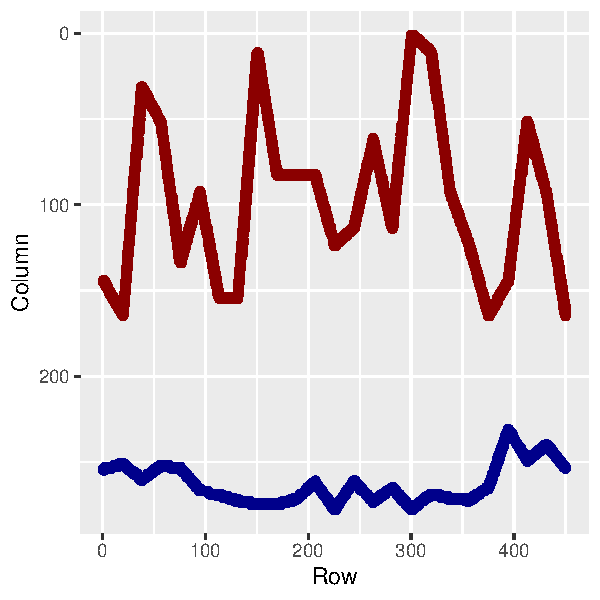
\includegraphics[width=4.0in]{IMAGENS/grafico_final}

\begin{center}
\tiny{}
\end{center}

\end{frame}

\begin{frame}[fragile]{Fraqueza na leitura de PDF}
\protect\hypertarget{fraqueza-na-leitura-de-pdf}{}

\begin{Shaded}
\begin{Highlighting}[]
\KeywordTok{require}\NormalTok{(pdftools)}
\NormalTok{tempo <-}\StringTok{ }\KeywordTok{image_read_pdf}\NormalTok{(}\StringTok{"IMAGENS/temp.pdf"}\NormalTok{)}
\KeywordTok{image_write}\NormalTok{(tempo, }\DataTypeTok{path =} \StringTok{"tempo.pdf"}\NormalTok{, }\DataTypeTok{format =} \StringTok{"pdf"}\NormalTok{)}
\end{Highlighting}
\end{Shaded}

\end{frame}

\begin{frame}{Fraqueza na leitura de PDF}
\protect\hypertarget{fraqueza-na-leitura-de-pdf-1}{}

\small

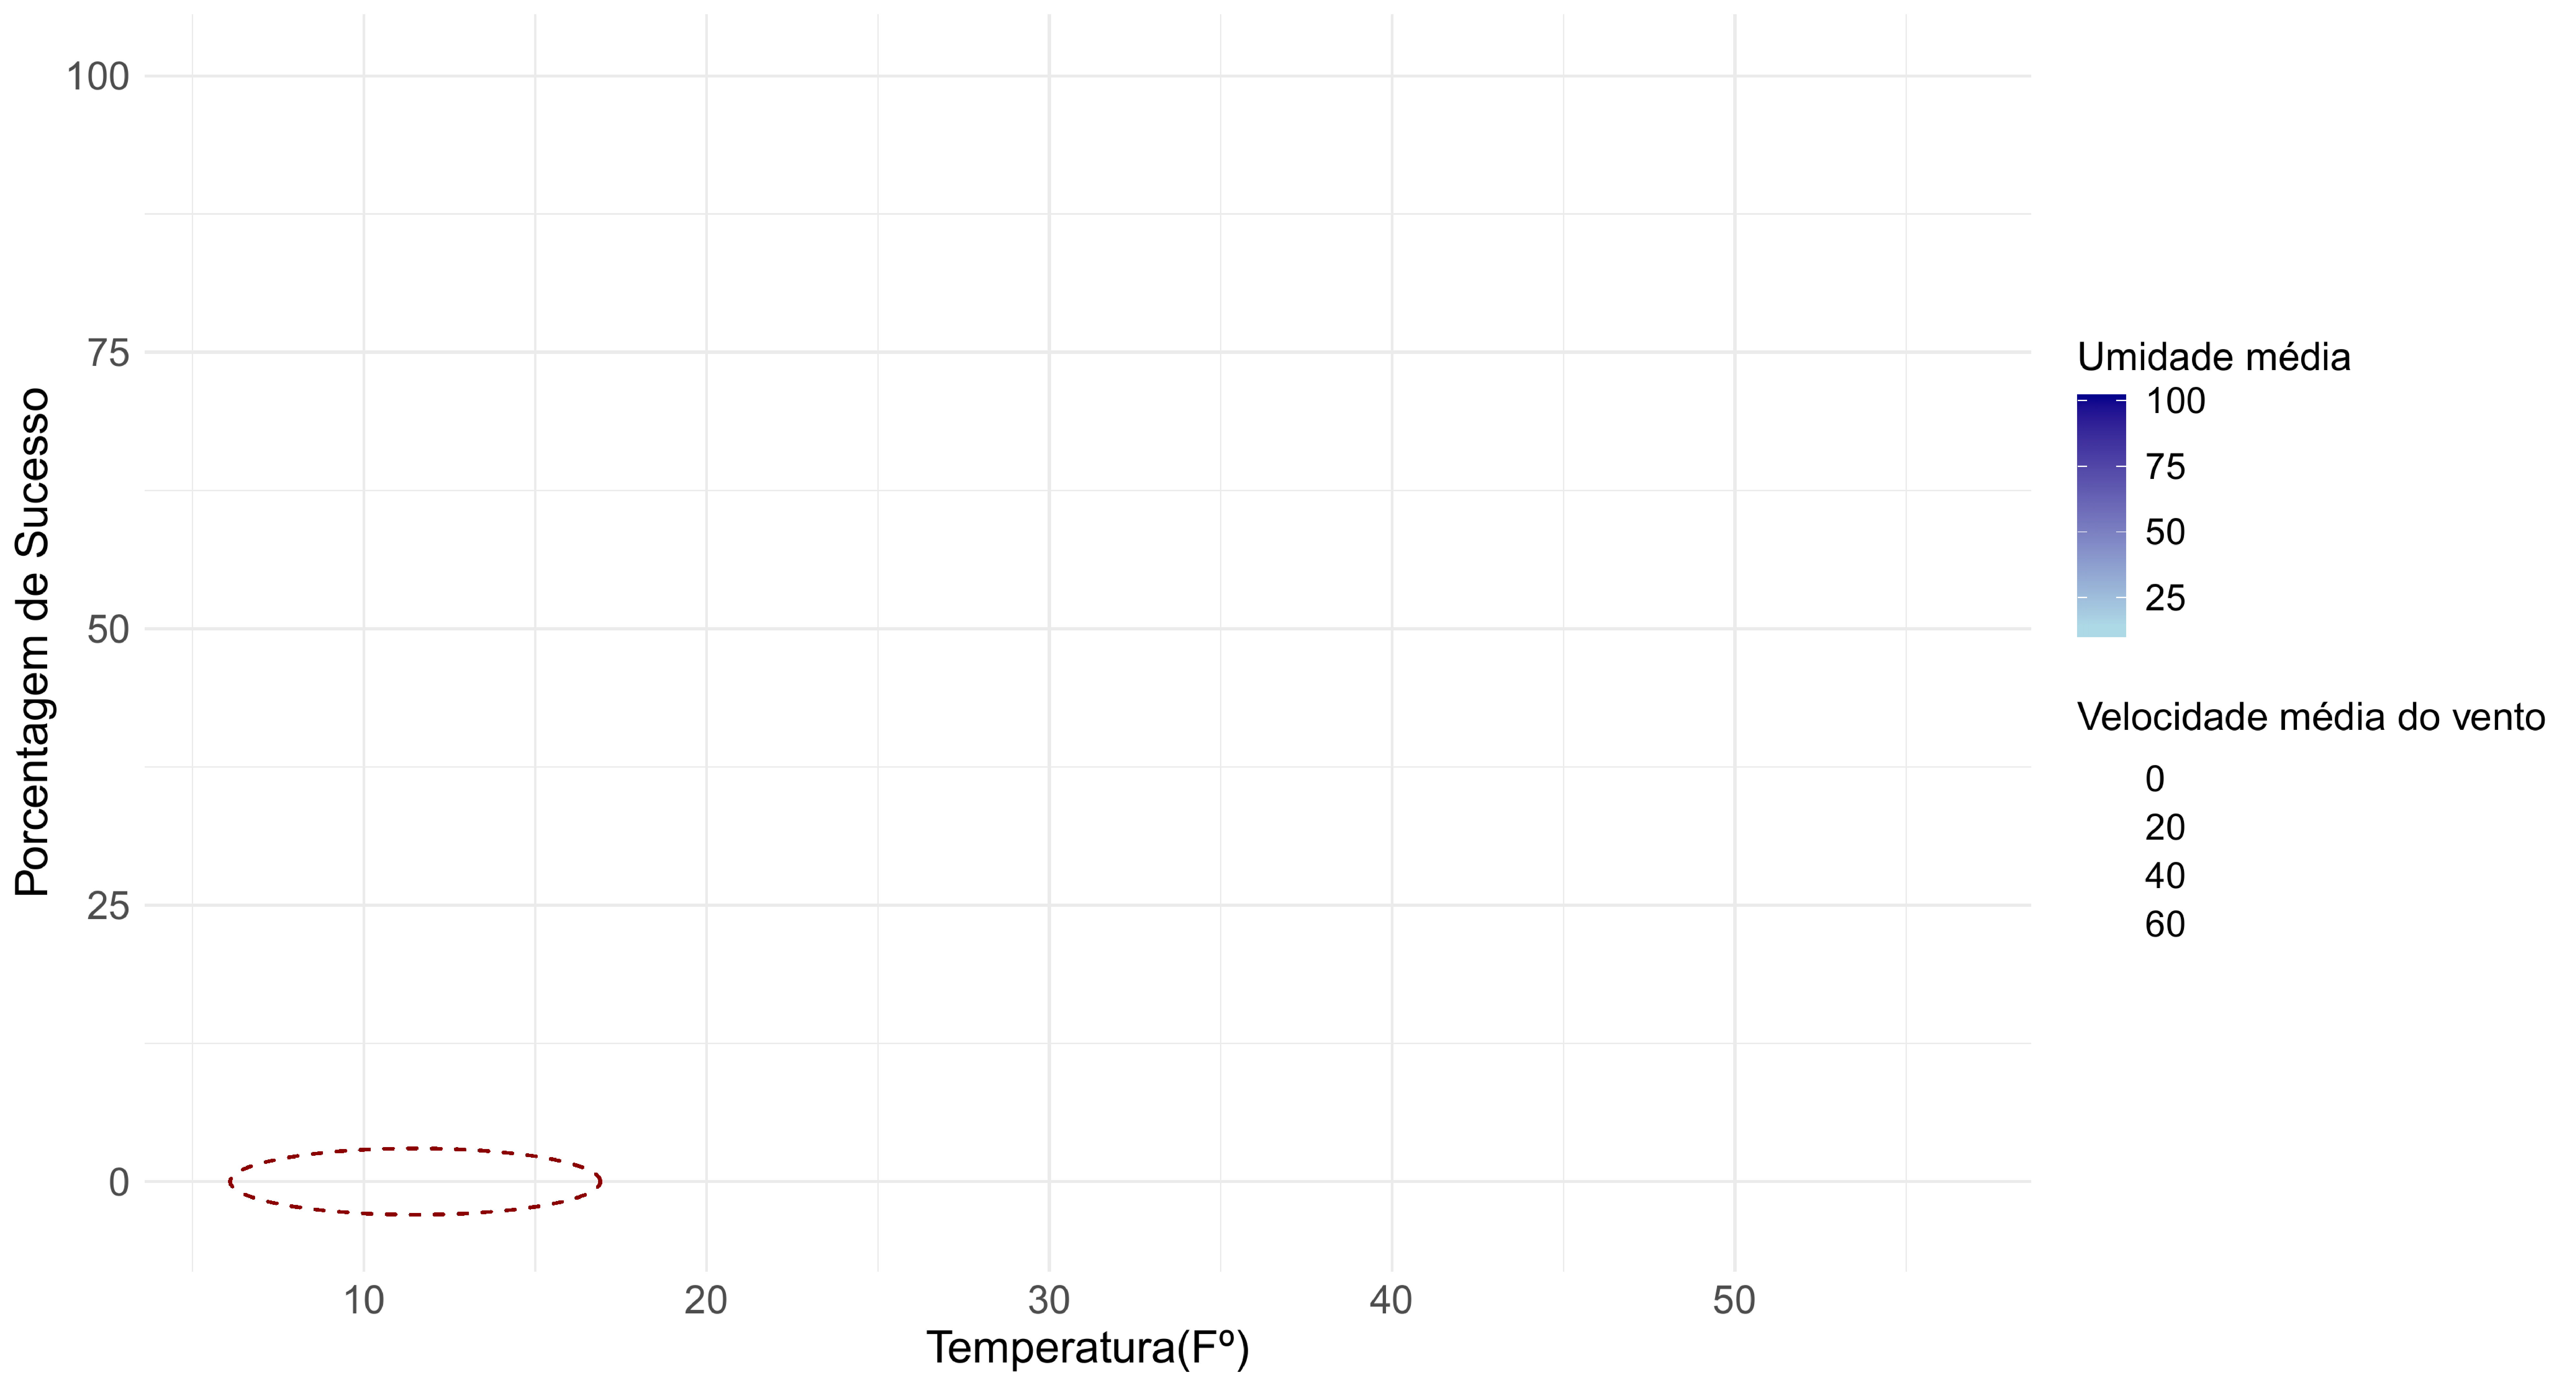
\includegraphics[width=4.0in]{tempo}

\begin{center}
\tiny{}
\end{center}

\end{frame}

\begin{frame}[fragile]{Gifs}
\protect\hypertarget{gifs}{}

\begin{Shaded}
\begin{Highlighting}[]
\NormalTok{earth <-}\StringTok{ }\KeywordTok{image_read}\NormalTok{(}
  \StringTok{"https://jeroen.github.io/images/earth.gif"}
\NormalTok{  ) }\OperatorTok
\StringTok{  }\KeywordTok{image_scale}\NormalTok{(}\StringTok{"250x"}\NormalTok{) }\OperatorTok\StringTok{ }
\StringTok{  }\KeywordTok{image_quantize}\NormalTok{() }

\KeywordTok{length}\NormalTok{(earth) }
\end{Highlighting}
\end{Shaded}

\begin{verbatim}
## [1] 44
\end{verbatim}

\end{frame}

\begin{frame}{Como montar um GIF}
\protect\hypertarget{como-montar-um-gif}{}

1º - Importe as imagens:

\(\Rightarrow\) im\_1 \textless-
image\_read(``C:/Users/nick\_/Downloads/im\_1.jpg'')

\(\Rightarrow\) im\_n \textless-
image\_read(``C:/Users/nick\_/Downloads/im\_n.jpg'')

2º - Junte as imagens e redimensione:

\(\Rightarrow\) img \textless- c(im\_1, \ldots{} , im\_n)

\(\Rightarrow\) img \textless- image\_scale(img, ``300x300'')

3º - Argumentos:

\(\Rightarrow\) image\_animate(img)

\end{frame}

\begin{frame}[fragile]{Salvar o GIF na máquina}
\protect\hypertarget{salvar-o-gif-na-muxe1quina}{}

\begin{Shaded}
\begin{Highlighting}[]
\KeywordTok{library}\NormalTok{(gifski)}

\KeywordTok{image_write_gif}\NormalTok{(img, }\DataTypeTok{path =} \StringTok{"grafico.gif"}\NormalTok{)}
 \CommentTok{# É possivel adicionar um delay}
\KeywordTok{image_write_gif}\NormalTok{(img, }\DataTypeTok{path =} \StringTok{"grafico_delay.gif"}\NormalTok{,}
                \DataTypeTok{delay =} \DecValTok{1}\OperatorTok{/}\DecValTok{6}\NormalTok{)}
\end{Highlighting}
\end{Shaded}

\end{frame}

\begin{frame}[fragile]{GIF e filtro Voronoi}
\protect\hypertarget{gif-e-filtro-voronoi}{}

\small

\begin{Shaded}
\begin{Highlighting}[]
\CommentTok{# Download da imagem}
\NormalTok{file=}\StringTok{"http://ereaderbackgrounds.com/movies/bw/Imagem.jpg"}
\KeywordTok{download.file}\NormalTok{(file, }\DataTypeTok{destfile =} \StringTok{"imagem.jpg"}\NormalTok{, }\DataTypeTok{mode =} \StringTok{'wb'}\NormalTok{)}
\CommentTok{# Lê e converte para a escala de cinza}
\KeywordTok{load.image}\NormalTok{(}\StringTok{"C:/Users/nick_/Downloads/Imagem.jpg"}\NormalTok{) }\OperatorTok\StringTok{ }
\StringTok{  }\KeywordTok{grayscale}\NormalTok{() ->}\StringTok{ }\NormalTok{x}
\end{Highlighting}
\end{Shaded}

\end{frame}

\begin{frame}[fragile]{GIF e filtro Voronoi}
\protect\hypertarget{gif-e-filtro-voronoi-1}{}

\small

\begin{Shaded}
\begin{Highlighting}[]
\CommentTok{# Isso é apenas para definir os limites dos frames}
\NormalTok{x }\OperatorTok\StringTok{ }
\StringTok{  }\KeywordTok{as.data.frame}\NormalTok{() }\OperatorTok\StringTok{ }
\StringTok{  }\KeywordTok{group_by}\NormalTok{() }\OperatorTok\StringTok{ }
\StringTok{  }\KeywordTok{summarize}\NormalTok{(}\DataTypeTok{xmin=}\KeywordTok{min}\NormalTok{(x), }\DataTypeTok{xmax=}\KeywordTok{max}\NormalTok{(x),}
            \DataTypeTok{ymin=}\KeywordTok{min}\NormalTok{(y), }\DataTypeTok{ymax=}\KeywordTok{max}\NormalTok{(y)) }\OperatorTok\StringTok{ }
\StringTok{  }\KeywordTok{as.vector}\NormalTok{()->rw}
\end{Highlighting}
\end{Shaded}

\end{frame}

\begin{frame}[fragile]{GIF e filtro Voronoi}
\protect\hypertarget{gif-e-filtro-voronoi-2}{}

\small

\begin{Shaded}
\begin{Highlighting}[]
\CommentTok{# Filtra a imagem e converte para preto e branco}
\NormalTok{x }\OperatorTok
\StringTok{  }\KeywordTok{threshold}\NormalTok{(}\StringTok{"45%"}\NormalTok{) }\OperatorTok\StringTok{ }
\StringTok{  }\KeywordTok{as.cimg}\NormalTok{() }\OperatorTok\StringTok{ }
\StringTok{  }\KeywordTok{as.data.frame}\NormalTok{() ->}\StringTok{ }\NormalTok{df}
\end{Highlighting}
\end{Shaded}

\end{frame}

\begin{frame}[fragile]{GIF e filtro Voronoi}
\protect\hypertarget{gif-e-filtro-voronoi-3}{}

\small

\begin{Shaded}
\begin{Highlighting}[]
\CommentTok{# Função para calcular e plotar o diagrama de Voronoi,}
\CommentTok{# depende do tamanho da amostra}
\NormalTok{doPlot =}\StringTok{ }\ControlFlowTok{function}\NormalTok{(n)}
\NormalTok{\{}
  \CommentTok{# Diagrama de Voronoi}
\NormalTok{  df }\OperatorTok\StringTok{ }
\StringTok{    }\KeywordTok{sample_n}\NormalTok{(n, }\DataTypeTok{weight=}\NormalTok{(}\DecValTok{1}\OperatorTok{-}\NormalTok{value)) }\OperatorTok\StringTok{ }
\StringTok{    }\KeywordTok{select}\NormalTok{(x,y) }\OperatorTok\StringTok{ }
\StringTok{    }\KeywordTok{deldir}\NormalTok{(}\DataTypeTok{rw=}\NormalTok{rw, }\DataTypeTok{sort=}\OtherTok{TRUE}\NormalTok{) }\OperatorTok\StringTok{ }
\StringTok{    }\NormalTok{.}\OperatorTok{$}\NormalTok{dirsgs ->}\StringTok{ }\NormalTok{data}
\end{Highlighting}
\end{Shaded}

\end{frame}

\begin{frame}[fragile]{GIF e filtro Voronoi}
\protect\hypertarget{gif-e-filtro-voronoi-4}{}

\small

\begin{Shaded}
\begin{Highlighting}[]
 \CommentTok{# Isso é apenas para adicionar alguns alfas nas linhas,}
 \CommentTok{# depende da longitude}
\NormalTok{  data }\OperatorTok\StringTok{ }
\StringTok{    }\KeywordTok{mutate}\NormalTok{(}\DataTypeTok{long=}\KeywordTok{sqrt}\NormalTok{((x1}\OperatorTok{-}\NormalTok{x2)}\OperatorTok{^}\DecValTok{2}\OperatorTok{+}\NormalTok{(y1}\OperatorTok{-}\NormalTok{y2)}\OperatorTok{^}\DecValTok{2}\NormalTok{),}
           \DataTypeTok{alpha=}\KeywordTok{findInterval}\NormalTok{(}
\NormalTok{             long,}
             \KeywordTok{quantile}\NormalTok{(long,}
                      \DataTypeTok{robs =} \KeywordTok{seq}\NormalTok{(}\DecValTok{0}\NormalTok{,}
                                 \DecValTok{1}\NormalTok{,}
                                 \DataTypeTok{length.out =} \DecValTok{20}\NormalTok{)}
\NormalTok{                                       )}
\NormalTok{                              )}\OperatorTok{/}\DecValTok{21}\NormalTok{)->}\StringTok{ }\NormalTok{data}
\end{Highlighting}
\end{Shaded}

\end{frame}

\begin{frame}[fragile]{GIF e filtro Voronoi}
\protect\hypertarget{gif-e-filtro-voronoi-5}{}

\small

\begin{Shaded}
\begin{Highlighting}[]
\NormalTok{data }\OperatorTok\StringTok{ }
\StringTok{    }\KeywordTok{ggplot}\NormalTok{(}\KeywordTok{aes}\NormalTok{(}\DataTypeTok{alpha=}\NormalTok{(}\DecValTok{1}\OperatorTok{-}\NormalTok{alpha))) }\OperatorTok{+}
\StringTok{    }\KeywordTok{geom_segment}\NormalTok{(}\KeywordTok{aes}\NormalTok{(}\DataTypeTok{x =}\NormalTok{ x1, }\DataTypeTok{y =}\NormalTok{ y1, }\DataTypeTok{xend =}\NormalTok{ x2, }\DataTypeTok{yend =}\NormalTok{ y2),}
                 \DataTypeTok{color=}\StringTok{"black"}\NormalTok{, }\DataTypeTok{lwd=}\DecValTok{1}\NormalTok{) }\OperatorTok{+}
\StringTok{    }\KeywordTok{scale_x_continuous}\NormalTok{(}\DataTypeTok{expand=}\KeywordTok{c}\NormalTok{(}\DecValTok{0}\NormalTok{,}\DecValTok{0}\NormalTok{))}\OperatorTok{+}
\StringTok{    }\KeywordTok{scale_y_continuous}\NormalTok{(}\DataTypeTok{expand=}\KeywordTok{c}\NormalTok{(}\DecValTok{0}\NormalTok{,}\DecValTok{0}\NormalTok{), }\DataTypeTok{trans=}\KeywordTok{reverse_trans}\NormalTok{())}\OperatorTok{+}
\StringTok{    }\KeywordTok{theme}\NormalTok{(}\DataTypeTok{legend.position  =} \StringTok{"none"}\NormalTok{,}
          \DataTypeTok{panel.background =} \KeywordTok{element_rect}\NormalTok{(}\DataTypeTok{fill=}\StringTok{"white"}\NormalTok{),}
          \DataTypeTok{axis.ticks       =} \KeywordTok{element_blank}\NormalTok{(),}
          \DataTypeTok{panel.grid       =} \KeywordTok{element_blank}\NormalTok{(),}
          \DataTypeTok{axis.title       =} \KeywordTok{element_blank}\NormalTok{(),}
          \DataTypeTok{axis.text        =} \KeywordTok{element_blank}\NormalTok{())->plot}
  \KeywordTok{return}\NormalTok{(plot)}\ErrorTok{\}}
\end{Highlighting}
\end{Shaded}

\end{frame}

\begin{frame}[fragile]{GIF e filtro Voronoi}
\protect\hypertarget{gif-e-filtro-voronoi-6}{}

\small

\begin{Shaded}
\begin{Highlighting}[]
\CommentTok{# Eu chamei a função anterior e salvei o resultado do plot em}
\CommentTok{# formato jpeg}
\NormalTok{i=}\StringTok{ }\DecValTok{500}
\NormalTok{name=}\KeywordTok{paste0}\NormalTok{(}\StringTok{"imagem"}\NormalTok{,i,}\StringTok{".jpeg"}\NormalTok{)}
\KeywordTok{jpeg}\NormalTok{(name, }\DataTypeTok{width =} \DecValTok{600}\NormalTok{, }\DataTypeTok{height =} \DecValTok{800}\NormalTok{, }\DataTypeTok{units =} \StringTok{"px"}\NormalTok{,}
     \DataTypeTok{quality =} \DecValTok{100}\NormalTok{)}
\KeywordTok{doPlot}\NormalTok{(i)}
\KeywordTok{dev.off}\NormalTok{()}
\end{Highlighting}
\end{Shaded}

\end{frame}

\begin{frame}[fragile]{GIF e filtro Voronoi}
\protect\hypertarget{gif-e-filtro-voronoi-7}{}

\small

\begin{Shaded}
\begin{Highlighting}[]
\CommentTok{# Assim que todas as imagens são salvas, eu posso criar o GIF}
\KeywordTok{library}\NormalTok{(magick)}
\NormalTok{frames=}\KeywordTok{c}\NormalTok{()}
\NormalTok{images=}\KeywordTok{list.files}\NormalTok{(}\DataTypeTok{pattern=}\StringTok{"jpeg"}\NormalTok{)}
\ControlFlowTok{for}\NormalTok{ (i }\ControlFlowTok{in} \KeywordTok{length}\NormalTok{(images)}\OperatorTok{:}\DecValTok{1}\NormalTok{)}
\NormalTok{\{}
\NormalTok{  x=}\KeywordTok{image_read}\NormalTok{(images[i])}
\NormalTok{  x=}\KeywordTok{image_scale}\NormalTok{(x, }\StringTok{"300"}\NormalTok{)}
  \KeywordTok{c}\NormalTok{(x, frames) ->}\StringTok{ }\NormalTok{frames}
\NormalTok{\}}
\NormalTok{animation=}\KeywordTok{image_animate}\NormalTok{(frames, }\DataTypeTok{fps =} \DecValTok{2}\NormalTok{)}
\KeywordTok{image_write}\NormalTok{(animation, }\StringTok{"Imagem.gif"}\NormalTok{)}
\KeywordTok{print}\NormalTok{(animation)}
\end{Highlighting}
\end{Shaded}

\end{frame}

\begin{frame}{Filtro geométrico}
\protect\hypertarget{filtro-geomuxe9trico}{}

\small

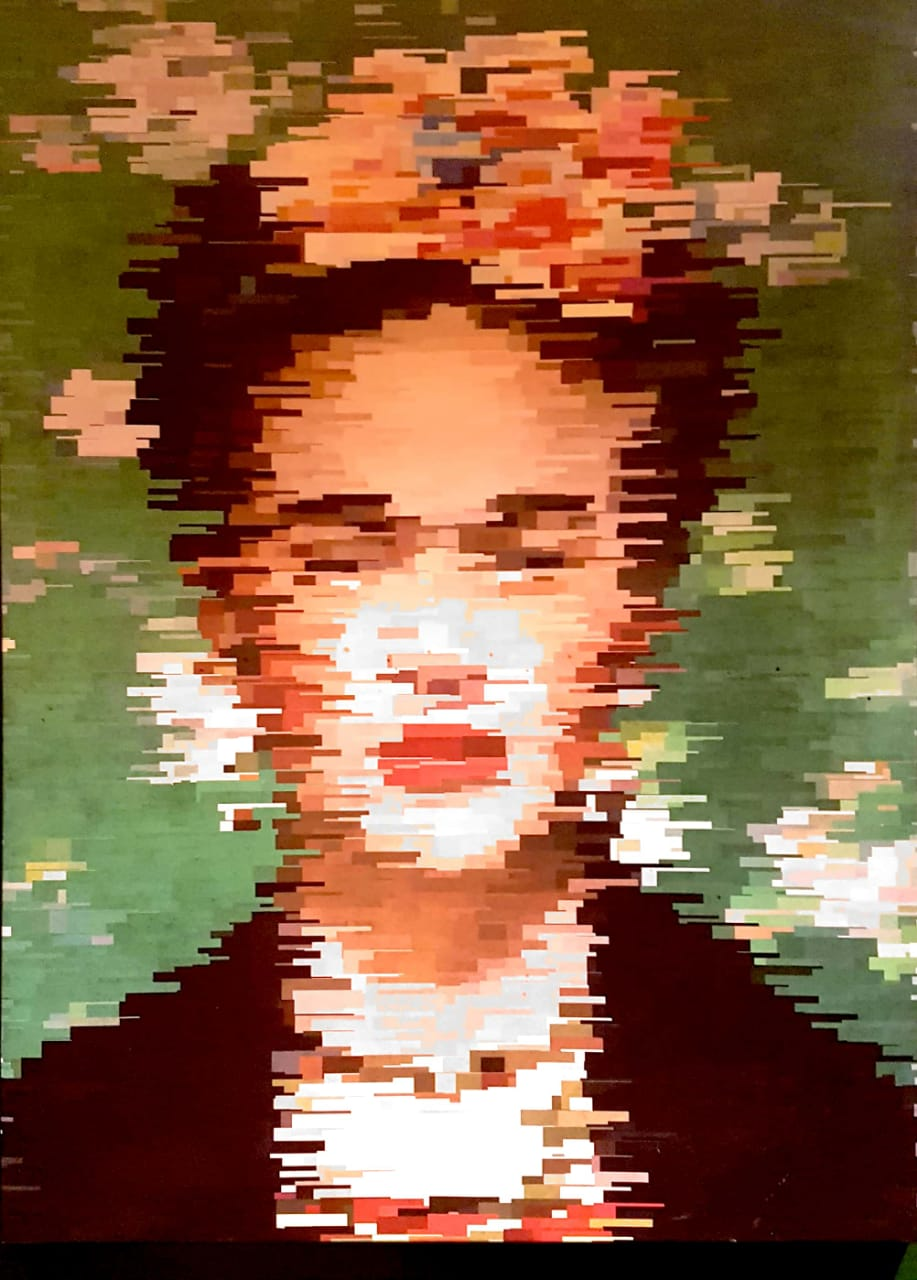
\includegraphics[width=4.5in]{IMAGENS/Frida}

\begin{center}
\tiny{}
\end{center}

\end{frame}

\begin{frame}[fragile]{Filtro geométrico}
\protect\hypertarget{filtro-geomuxe9trico-1}{}

\small

Por meio do pacote ``imager'' é possível estilizar uma imagem e deixá-la
pixelizada:

\begin{Shaded}
\begin{Highlighting}[]
\KeywordTok{library}\NormalTok{(imager)}
\NormalTok{foto <-}\StringTok{ }\KeywordTok{load.image}\NormalTok{(}\StringTok{"C:/Users/nick_/Downloads/foto.jpg"}\NormalTok{)}

\NormalTok{foto2<-}\StringTok{ }\NormalTok{foto }\OperatorTok\StringTok{  }\KeywordTok{resize}\NormalTok{(}\DataTypeTok{size_x =} \DecValTok{80}\NormalTok{, }\DataTypeTok{size_y =} \DecValTok{80}\NormalTok{,}
                         \DataTypeTok{interpolation_type =}\NormalTok{ 1L)}
\KeywordTok{suppressMessages}\NormalTok{(}\KeywordTok{suppressWarnings}\NormalTok{(}\KeywordTok{library}\NormalTok{(imager)))}
\NormalTok{foto2 <-}\StringTok{ }\KeywordTok{rowMeans}\NormalTok{(foto2, }\DataTypeTok{dims =} \DecValTok{2}\NormalTok{)}
\end{Highlighting}
\end{Shaded}

\end{frame}

\begin{frame}[fragile]{Filtro geométrico}
\protect\hypertarget{filtro-geomuxe9trico-2}{}

\small

\begin{Shaded}
\begin{Highlighting}[]
\NormalTok{foto2 }\OperatorTok
\StringTok{  }\KeywordTok{apply}\NormalTok{(}\DecValTok{1}\NormalTok{, rev) }\OperatorTok\StringTok{ }
\StringTok{  }\KeywordTok{t}\NormalTok{() }\OperatorTok\StringTok{ }
\StringTok{  }\KeywordTok{image}\NormalTok{(}\DataTypeTok{col =} \KeywordTok{grey.colors}\NormalTok{(}\DecValTok{256}\NormalTok{), }\DataTypeTok{axes =} \OtherTok{FALSE}\NormalTok{)}
\end{Highlighting}
\end{Shaded}

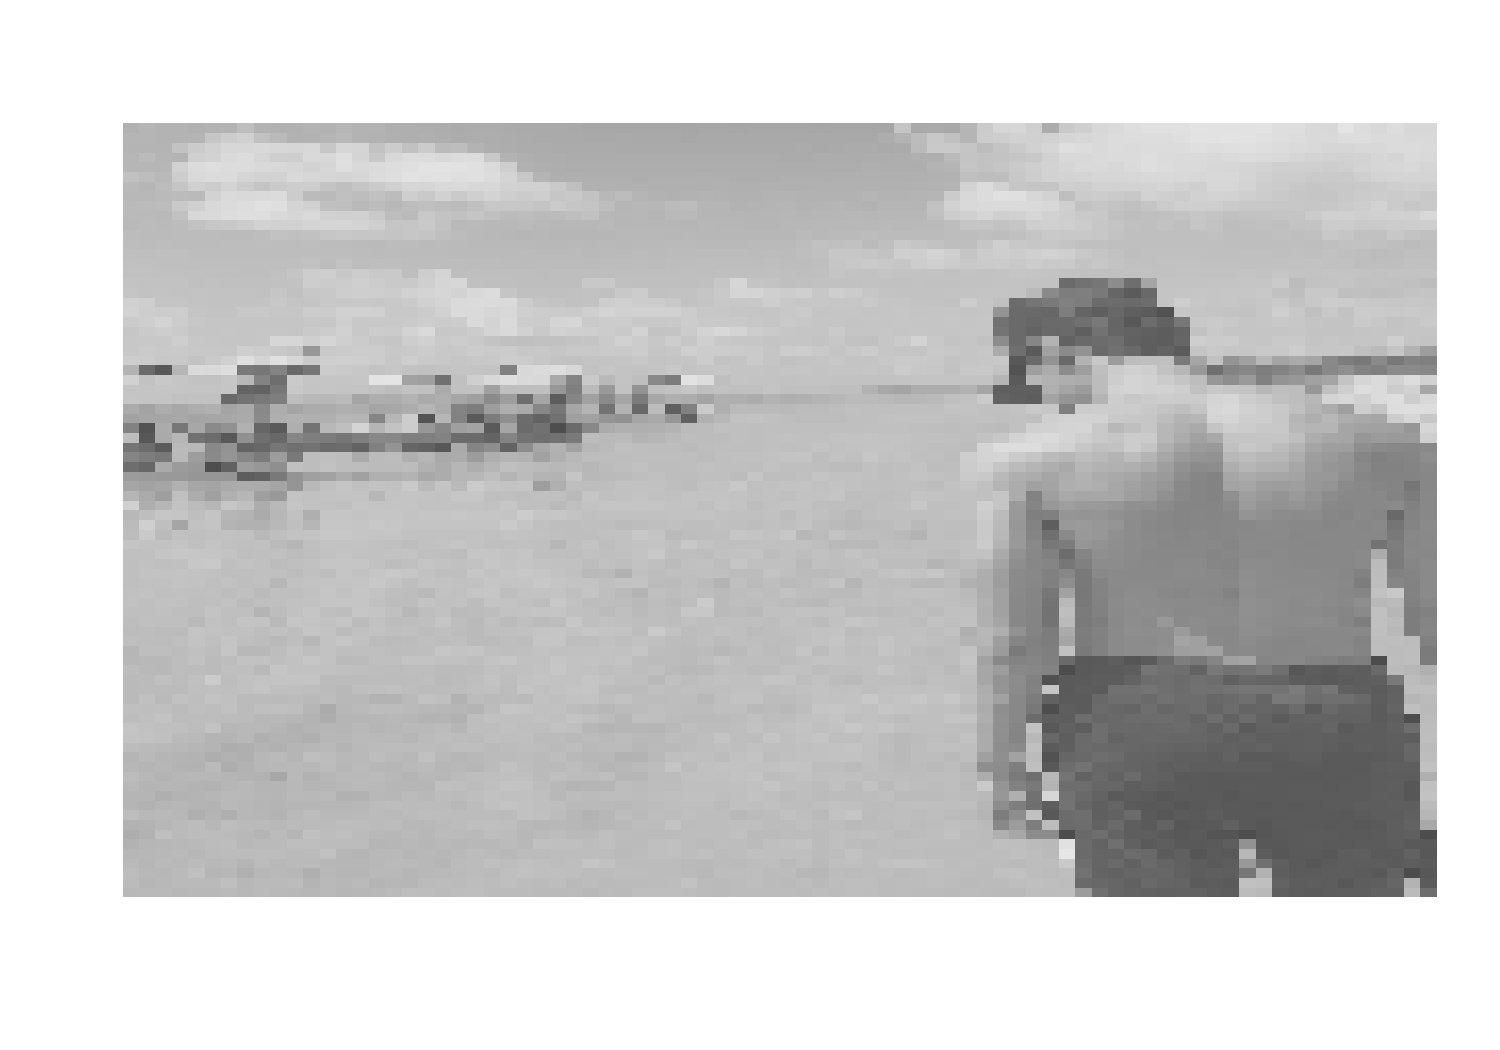
\includegraphics{SLIDES_files/figure-beamer/10.1-1.pdf}

\end{frame}

\begin{frame}{Keras}
\protect\hypertarget{keras}{}


\includegraphics[width=4.5in]{IMAGENS/Keras_logo}

\begin{center}
\tiny{}
\end{center}

\end{frame}

\begin{frame}{TensorFlow}
\protect\hypertarget{tensorflow}{}


\includegraphics[width=4.5in]{IMAGENS/TensorFlow_logo}

\begin{center}
\tiny{}
\end{center}

\end{frame}

\begin{frame}{Anaconda}
\protect\hypertarget{anaconda}{}


\includegraphics[width=4.2in]{IMAGENS/Anaconda}

\begin{center}
\tiny{}
\end{center}

\end{frame}

\begin{frame}{Reconhecimento de imagem - Aviões e carros}
\protect\hypertarget{reconhecimento-de-imagem---aviuxf5es-e-carros}{}

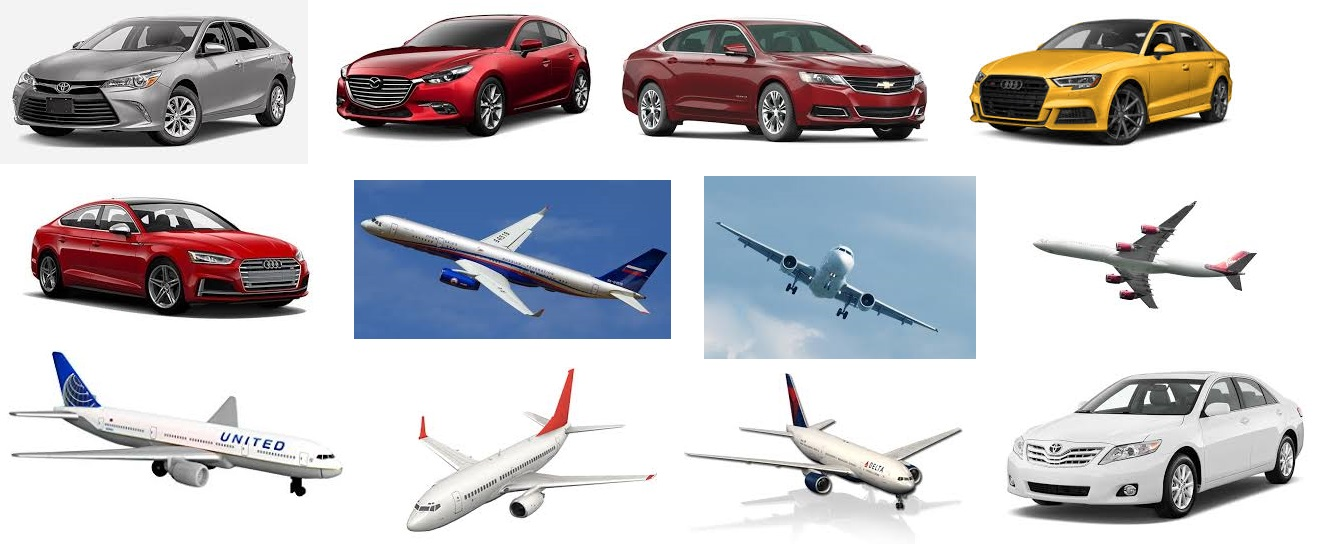
\includegraphics[width=4.0in]{IMAGENS/Avioes_carros}

\begin{center}
\tiny{}
\end{center}

\end{frame}

\begin{frame}[fragile]{Reconhecimento de imagem - Pacotes}
\protect\hypertarget{reconhecimento-de-imagem---pacotes}{}

\begin{Shaded}
\begin{Highlighting}[]
\KeywordTok{install.packages}\NormalTok{(}\StringTok{"tfestimators"}\NormalTok{)}
\KeywordTok{install_tensorflow}\NormalTok{()}
\NormalTok{devtools}\OperatorTok{::}\KeywordTok{install_github}\NormalTok{(}\StringTok{"rstudio/keras"}\NormalTok{)}
\NormalTok{devtools}\OperatorTok{::}\KeywordTok{install_github}\NormalTok{(}\StringTok{"rstudio/tensorflow"}\NormalTok{)}
\NormalTok{devtools}\OperatorTok{::}\KeywordTok{install_github}\NormalTok{(}\StringTok{"rstudio/keras"}\NormalTok{)}
\NormalTok{reticulate}\OperatorTok{::}\KeywordTok{py_discover_config}\NormalTok{()}
\NormalTok{reticulate}\OperatorTok{::}\KeywordTok{use_condaenv}\NormalTok{(}\StringTok{"r-tensorflow"}\NormalTok{)}
\NormalTok{reticulate}\OperatorTok{::}\KeywordTok{py_config}\NormalTok{()}
\end{Highlighting}
\end{Shaded}

\end{frame}

\begin{frame}[fragile]{Reconhecimento de imagem - Leitura}
\protect\hypertarget{reconhecimento-de-imagem---leitura}{}

\begin{Shaded}
\begin{Highlighting}[]
\KeywordTok{library}\NormalTok{(EBImage)}
\KeywordTok{library}\NormalTok{(keras)}
\KeywordTok{library}\NormalTok{(kerasR)}
\KeywordTok{library}\NormalTok{(kerasformula)}
\KeywordTok{setwd}\NormalTok{(}\StringTok{'C:}\CharTok{\textbackslash{}\textbackslash{}}\StringTok{Users}\CharTok{\textbackslash{}\textbackslash{}}\StringTok{diretorio R'}\NormalTok{)}
\NormalTok{pics <-}\StringTok{ }\KeywordTok{c}\NormalTok{(}\StringTok{'p1.jpg'}\NormalTok{, }\StringTok{'p2.jpg'}\NormalTok{, }\StringTok{'p3.jpg'}\NormalTok{, }\StringTok{'p4.jpg'}\NormalTok{, }\StringTok{'p5.jpg'}\NormalTok{,}
          \StringTok{'p6.jpg'}\NormalTok{,}\StringTok{'c1.jpg'}\NormalTok{, }\StringTok{'c2.jpg'}\NormalTok{, }\StringTok{'c3.jpg'}\NormalTok{, }\StringTok{'c4.jpg'}\NormalTok{, }
          \StringTok{'c5.jpg'}\NormalTok{,}\StringTok{'c6.jpg'}\NormalTok{)}
\NormalTok{mypic <-}\StringTok{ }\KeywordTok{list}\NormalTok{()}
\ControlFlowTok{for}\NormalTok{ (i }\ControlFlowTok{in} \DecValTok{1}\OperatorTok{:}\DecValTok{12}\NormalTok{) \{mypic[[i]] <-}\StringTok{ }\KeywordTok{readImage}\NormalTok{(pics[i])\}}
\end{Highlighting}
\end{Shaded}

\end{frame}

\begin{frame}[fragile]{Reconhecimento de imagem - Análise manual}
\protect\hypertarget{reconhecimento-de-imagem---anuxe1lise-manual}{}

\begin{Shaded}
\begin{Highlighting}[]
\KeywordTok{print}\NormalTok{(mypic[[}\DecValTok{1}\NormalTok{]])}
\KeywordTok{display}\NormalTok{(mypic[[}\DecValTok{12}\NormalTok{]])}
\KeywordTok{summary}\NormalTok{(mypic[[}\DecValTok{1}\NormalTok{]])}
\KeywordTok{hist}\NormalTok{(mypic[[}\DecValTok{2}\NormalTok{]])}
\end{Highlighting}
\end{Shaded}

\end{frame}

\begin{frame}[fragile]{Reconhecimento de imagem - Redimensionamento}
\protect\hypertarget{reconhecimento-de-imagem---redimensionamento}{}

\begin{Shaded}
\begin{Highlighting}[]
\ControlFlowTok{for}\NormalTok{ (i }\ControlFlowTok{in} \DecValTok{1}\OperatorTok{:}\DecValTok{12}\NormalTok{) \{mypic[[i]] <-}\StringTok{ }\KeywordTok{resize}\NormalTok{(mypic[[i]],}\DecValTok{28}\NormalTok{, }\DecValTok{28}\NormalTok{)\}}
\ControlFlowTok{for}\NormalTok{ (i }\ControlFlowTok{in} \DecValTok{1}\OperatorTok{:}\DecValTok{12}\NormalTok{) \{mypic[[i]] <-}\StringTok{ }\KeywordTok{array_reshape}\NormalTok{(mypic[[i]],}
                                             \KeywordTok{c}\NormalTok{(}\DecValTok{28}\NormalTok{,}\DecValTok{28}\NormalTok{,}\DecValTok{3}\NormalTok{))\}}
\end{Highlighting}
\end{Shaded}

\end{frame}

\begin{frame}[fragile]{Reconhecimneto de imagem - Remodelagem}
\protect\hypertarget{reconhecimneto-de-imagem---remodelagem}{}

\begin{Shaded}
\begin{Highlighting}[]
\NormalTok{trainx <-}\StringTok{ }\OtherTok{NULL}
\ControlFlowTok{for}\NormalTok{ (i }\ControlFlowTok{in} \DecValTok{1}\OperatorTok{:}\DecValTok{5}\NormalTok{) \{trainx <-}\StringTok{ }\KeywordTok{rbind}\NormalTok{(trainx, mypic[[i]])\}}
\ControlFlowTok{for}\NormalTok{ (i }\ControlFlowTok{in} \DecValTok{7}\OperatorTok{:}\DecValTok{11}\NormalTok{) \{trainx <-}\StringTok{ }\KeywordTok{rbind}\NormalTok{(trainx, mypic[[i]])\}}
\KeywordTok{str}\NormalTok{(trainx)}
\NormalTok{testx <-}\StringTok{ }\KeywordTok{rbind}\NormalTok{(mypic[[}\DecValTok{6}\NormalTok{]], mypic[[}\DecValTok{12}\NormalTok{]])}
\NormalTok{trainy <-}\StringTok{ }\KeywordTok{c}\NormalTok{(}\DecValTok{0}\NormalTok{,}\DecValTok{0}\NormalTok{,}\DecValTok{0}\NormalTok{,}\DecValTok{0}\NormalTok{,}\DecValTok{0}\NormalTok{,}\DecValTok{1}\NormalTok{,}\DecValTok{1}\NormalTok{,}\DecValTok{1}\NormalTok{,}\DecValTok{1}\NormalTok{,}\DecValTok{1}\NormalTok{)}
\NormalTok{testy <-}\StringTok{ }\KeywordTok{c}\NormalTok{(}\DecValTok{0}\NormalTok{, }\DecValTok{1}\NormalTok{)}
\end{Highlighting}
\end{Shaded}

\end{frame}

\begin{frame}[fragile]{Reconhecimneto de imagem - Criação de labels}
\protect\hypertarget{reconhecimneto-de-imagem---criauxe7uxe3o-de-labels}{}

\begin{Shaded}
\begin{Highlighting}[]
\NormalTok{trainLabels <-}\StringTok{ }\KeywordTok{to_categorical}\NormalTok{(trainy)}
\NormalTok{testLabels <-}\StringTok{ }\KeywordTok{to_categorical}\NormalTok{(testy)}
\end{Highlighting}
\end{Shaded}

\end{frame}

\begin{frame}[fragile]{Reconhecimento de imagem - Modelo}
\protect\hypertarget{reconhecimento-de-imagem---modelo}{}

\begin{Shaded}
\begin{Highlighting}[]
\NormalTok{model <-}\StringTok{ }\KeywordTok{keras_model_sequential}\NormalTok{()}
\NormalTok{model }\OperatorTok
\StringTok{         }\KeywordTok{layer_dense}\NormalTok{(}\DataTypeTok{units =} \DecValTok{256}\NormalTok{, }\DataTypeTok{activation =} \StringTok{'relu'}\NormalTok{,}
                     \DataTypeTok{input_shape =} \KeywordTok{c}\NormalTok{(}\DecValTok{2352}\NormalTok{)) }\OperatorTok
\StringTok{         }\KeywordTok{layer_dense}\NormalTok{(}\DataTypeTok{units =} \DecValTok{128}\NormalTok{, }\DataTypeTok{activation =} \StringTok{'relu'}\NormalTok{) }\OperatorTok
\StringTok{         }\KeywordTok{layer_dense}\NormalTok{(}\DataTypeTok{units =} \DecValTok{2}\NormalTok{, }\DataTypeTok{activation =} \StringTok{'softmax'}\NormalTok{)}
\KeywordTok{summary}\NormalTok{(model)}
\end{Highlighting}
\end{Shaded}

\end{frame}

\begin{frame}[fragile]{Reconhecimento de imagem - Compilação}
\protect\hypertarget{reconhecimento-de-imagem---compilauxe7uxe3o}{}

\begin{Shaded}
\begin{Highlighting}[]
\NormalTok{model }\OperatorTok
\StringTok{         }\KeywordTok{compile}\NormalTok{(}\DataTypeTok{loss =} \StringTok{'binary_crossentropy'}\NormalTok{,}
                 \DataTypeTok{optimizer =} \KeywordTok{optimizer_rmsprop}\NormalTok{(),}
                 \DataTypeTok{metrics =} \StringTok{'accuracy'}\NormalTok{)}
\end{Highlighting}
\end{Shaded}

\end{frame}

\begin{frame}[fragile]{Reconhecimento de imagem - Ajustando/ Treinando o
modelo}
\protect\hypertarget{reconhecimento-de-imagem---ajustando-treinando-o-modelo}{}

\begin{Shaded}
\begin{Highlighting}[]
\NormalTok{history <-}\StringTok{ }\NormalTok{model }\OperatorTok
\StringTok{         }\KeywordTok{fit}\NormalTok{(trainx,}
\NormalTok{             trainLabels,}
             \DataTypeTok{epochs =} \DecValTok{500}\NormalTok{,}
             \DataTypeTok{batch_size =} \DecValTok{32}\NormalTok{,}
             \DataTypeTok{validation_split =} \FloatTok{0.2}\NormalTok{)}
\end{Highlighting}
\end{Shaded}

\end{frame}

\begin{frame}{Reconhecimento de imagem - Ajustando/ Treinando o modelo}
\protect\hypertarget{reconhecimento-de-imagem---ajustando-treinando-o-modelo-1}{}

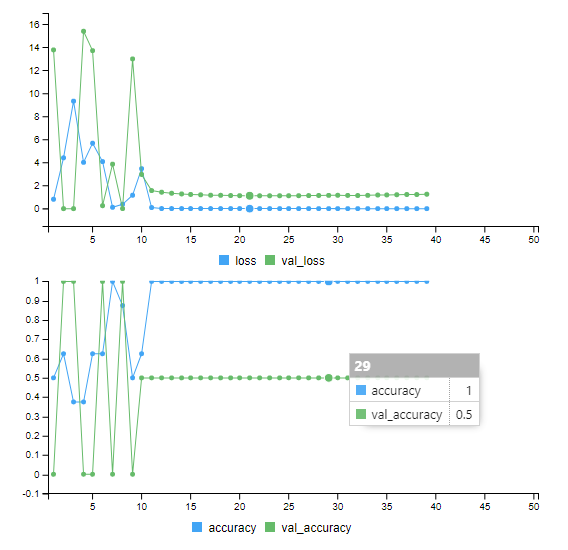
\includegraphics[width=3.2in]{IMAGENS/modelo_grafico}

\begin{center}
\tiny{}
\end{center}

\end{frame}

\begin{frame}[fragile]{Reconhecimento de imagem - Avaliação e previsão}
\protect\hypertarget{reconhecimento-de-imagem---avaliauxe7uxe3o-e-previsuxe3o}{}

\begin{Shaded}
\begin{Highlighting}[]
\NormalTok{model }\OperatorTok\StringTok{ }\KeywordTok{evaluate}\NormalTok{(testx, testLabels)}
\NormalTok{pred <-}\StringTok{ }\NormalTok{model }\OperatorTok\StringTok{ }\KeywordTok{predict_classes}\NormalTok{(trainx)}
\KeywordTok{table}\NormalTok{(}\DataTypeTok{Predicted =}\NormalTok{ pred, }\DataTypeTok{Actual =}\NormalTok{ trainy)}
\NormalTok{prob <-}\StringTok{ }\NormalTok{model }\OperatorTok\StringTok{ }\KeywordTok{predict_proba}\NormalTok{(trainx)}
\KeywordTok{cbind}\NormalTok{(prob, }\DataTypeTok{Prected =}\NormalTok{ pred, }\DataTypeTok{Actual=}\NormalTok{ trainy)}
\end{Highlighting}
\end{Shaded}

\end{frame}

\end{document}
